%\documentclass[draft,landscape, 11pt, oneside]{report}
\documentclass[landscape, 11pt, oneside, twoside]{report}
\usepackage[a4paper, left=1cm, right=1cm, top=2.5cm]{geometry}
\usepackage{lmodern}
\usepackage{hyperref}
\usepackage{titlesec}
\usepackage{scrextend}
\usepackage{array}
\usepackage{ProphetPanel}
\usepackage{fontspec}
\usepackage[T1]{fontenc}
\usepackage{longtable}
\usepackage{ProphetTerms}
\usepackage{float}
\usepackage{setspace}
%\usepackage[inline]{showlabels}
\setmainfont[
 BoldFont={FiraSans-Bold}, 
 ItalicFont={FiraSans-Italic},
 ]{FiraSans}
\setlength{\parindent}{0pt}
\setlength{\parskip}{1em}
\setlength{\evensidemargin}{0cm}
\setlength{\oddsidemargin}{2cm}
\setlength{\paperheight}{210mm}
\setlength{\paperwidth}{297mm}
\setlength{\textwidth}{22cm}
\setlength{\footskip}{2.5cm}
%\input{defined_terms.tex}
\newenvironment{flowtext}{\addmargin[0cm]{0cm}}{\endaddmargin} % standard text width (reduced for layout)
\newcommand{\pp}[1]{} % patch parameter
\newcommand{\app}[2]{} % additional patch parameter, 1: number, 2: name


%%\title{[DRAFT] User Manual for the GliGli upgraded Prophet-600}
%%\pagestyle{myheadings}\markright{[DRAFT] User Manual for the GliGli upgraded Prophet-600}
%%\makeatletter
%%\renewcommand\chapter{\pagestyle{myheadings}\markright{[DRAFT] User Manual for the GliGli upgraded Prophet-600}\global\@topnum\z@\@afterindentfalse\secdef\@chapter\@schapter}
%%\makeatother
\titleformat{\chapter}[display]{\LARGE\bfseries}{}{0.0cm}{}
\titlespacing{\chapter}{0pt}{*0}{*0}
\titlespacing{\section}{0pt}{*0}{*0}


%%
%% Document Start
%%


\begin{document}

\raggedbottom
\singlespacing

\begin{titlepage}
\pagenumbering{gobble}

% this it the title "Prophet-600"
  \begin{tikzpicture}[scale=0.8]
    \begin{scope}[xslant=0.1]
        \SSGBit[1.5cm]{0,0}{12567}
        \SSGBit[1.5cm]{2.5cm,0}{57}
        \SSGBit[1.5cm]{5cm,0}{5734}
        \SSGBit[1.5cm]{7.5,0}{12567}
        \SSGBit[1.5cm]{10cm,0}{3567}
        \SSGBit[1.5cm]{12.5cm,0}{14567}
        \SSGBit[1.5cm]{15cm,0}{4567}
        \SSGBit[1.5cm]{17.5cm,0}{7}
        \SSGBit[1.5cm]{20cm,0}{134567}
        \SSGBit[1.5cm]{22.5cm,0}{123456}
        \SSGBit[1.5cm]{25cm,0}{123456}
      \end{scope}
  \end{tikzpicture}

  \vspace{1cm}
  
  
  \Huge
  User Manual \vspace{0.4cm} \\
  \Large
  Edition: version v2022 (8.8.2022) \vspace{0.3cm}\\
  Firmware version: GliGli \version by imogen\vspace{0.3cm}\\
  Editor / author: imogen / image-et-son 
  \normalsize

\end{titlepage}


\pagebreak
\pagebreak

%\maketitle
\tableofcontents


\pagestyle{myheadings}\markright{Prophet-600 \version User Manual }
\makeatletter
\renewcommand\chapter{\pagestyle{myheadings}\markright{Prophet-600 \version User Manual}\global\@topnum\z@\@afterindentfalse\secdef\@chapter\@schapter}
\makeatother

\pagebreak
\chapter{Introduction to the GliGli Prophet-600 Firmware Upgrade}

\pagenumbering{arabic}
\setcounter{page}{1}

\begin{flowtext}

The original Sequential Circuits Prophet-600 from around 1982 is run by a Zilog Z80 processor. This processor (and the firmware written for it) is pushed beyond its limits for computing and applying the voltages, for scanning user inputs and managing MIDI events. The necessary compromises made the instrument steppy, glitchy and non-responsive. That is a pity, because the basic synth voice hardware of the Prophet-600 is good: unlike DCO synths which became popular and affordable at the time, the Prophet-600 is a 6 voice analog synthesizer driven by 2 voltage controlled oscillators (VCOs) and a 24db low pass filter per voice, all implemented using the renowned Curtis chips \cite{curtis}. The hardware also provides hard sync, frequency modulation and even modulation of cut-off by VCO. It is very versatile. The shortcomings of the original Prophet-600 were due only to the unfortunate circumstance that the selected and commonly available micro-processors at the time were not powerful enough for the Prophet-600. So the idea to make use of a more modern processor 30 years later was interesting. Around 2013 GliGli \cite{gligli} started reverse engineering the original firmware for the Z80 and found that the Z80 can be replaced by a (more) modern Teensy++ 2.0 USB programmable microprocessor \cite{teensy} (with some hardware modifications). This was the start of what is now know as the \textit{Prophet-600 GliGli firmware upgrade}. GliGli describes his motivation as follows:

\begin{addmargin}[2cm]{1cm}

\textit{I love vintage analog synthesizers, and to be honest, my dream synth would be a Prophet-5, but when I heard what the Prophet-600 was capable of tone wise, I immediately thought its major weaknesses -- the lousy computer part, software envelopes and LFO -- could become its strength with a remake; basically the whole internal synth in voltage-controlled from a nice 14bit DAC, so with a fast modern micro controller, it could become awesome, maybe even better than a Prophet-5!}

\end{addmargin}

There are various modifications and modern CPU "implants" for some vintage analog synthesizers. Since the Teensy++ 2.0 board fits in to the same 2x20 pin standard socket of the Z80, the decisive advantage of the GliGli approach is that it is an easy-to-install and non-destructive firmware drop-in replacement\footnote{There are two versions of the Prophet-600. One has the Z80 on a socket. In this case replacement is truly "drop-in". The other version has the Z80 soldered to the circuit board. In this case the Z80 needs to be removed and a socket has to be soldered in its place first.}. It is completely safe to try out the Teensy++ 2.0 upgrade because one can always remove the board and restore the Z80 without technical expertise or training. 

The Teensy++ 2.0 offers completely new possibilities. Just looking at specs: the Z80 version of the Prophet-600 ran at 4 MHz while the ATMEL processor on the Teensy board is operated at 16 MHz. Also, the on-board flash memory provides much better storage and firmware handling possibilities compared to the EPROM which the Z80 uses. The firmware does not rely on a battery for keeping patch data in memory. With the replacement the obvious limitations of the original Prophet-600 could be overcome - but more than that, it opened the possibility for new and for enhanced features. 

Developing the software was a major effort with low-level functions and basic hardware communication at the core, e.g. instruction to set voltages to the electronic components, MIDI (interrupt) implementation, multiplexer operations and DAC operations. On top of this there is the "musical" part of coding such as envelopes, LFOs, modulations and sequencing functions as well as UI functions. Many people have contributed, most probably out of curiosity and passion for synthesizers and driven by the excitement that such a project could not only be conjured up but also be implemented and brought to life. 

The first stable version of the firmware upgrade was version 2.0 in 2014. An intermediate release (or at least something close to a release) version 2.1 Release Candidate 3 (2.1 RC3) has been available from September 5th 2015 on GliGli's webpages \cite{gligli}. The latest release version \version is the result of continued development between September 2021 and March 2022. It is meant as a celebration and revival of the original idea and it provides various new features and also significant improvements in core functions. The latest firmware version can be found on the project page\cite{newversion}.

While there is a realistic backlog of additional ideas to come in the future, there is a clear end of Prophet-600 upgrade story in sight because of ultimate hardware limitations. Firstly, PJRC (the manufacturer of the Teensy boards) has stopped producing the Teensy++ 2.0 board, so that it has become difficult to find them. Secondly, after extensive performance testing in the latest firmware developments efforts, it has become clear that the performance (smoothness and responsiveness of controls, timely and accurate processing of information) is finally limited by the built-in hardware, in particular the DAC (limited by voltage rise times) and multiplexer (limited by switching times). 

If you own a Teensy++ 2.0 upgraded Prophet-600 you can still enjoy some exciting new developments. The following is a compact summary of the improved and the new features. The manual generally refers to the latest version \version. Differences between versions are marked or commented in the text for your information. Share the passion for analog synthesizers with the Prophet-600 upgrade story!  

\begin{flushright}
  \textit{imogen / image-et-son}
\end{flushright}

\pagebreak
\section{What you can expect from the Firmware Upgrade}

\textbf{General features compared to the original Z80 version}
  
\begin{itemize}
  \setlength\itemsep{0cm}
  \item Greater resolution of many of the sound parameters with an improved refresh rate that makes the instrument much more responsive, again improved in \version using a dynamic scheme for reading user controls.
  \item Faster and smoother ADSR envelopes with support for two speed regimes (slow, fast) and two shapes (linear, exponential). The latest version \version has new linear shapes which were inspired by Prophet-5 rev 1/2 envelopes and designed to be more organic and musical than the former linear shapes.
  \item Positive and negative envelope amount settings for filter and poly-mod 
  \item A new LFO function generator with a wider frequency range from one cycle every 20 seconds to about 60Hz
  \item Assignable, random and up/down arpeggiator, optionally sync-able to external MIDI and analog clock
  \item Multiple note assignment modes including last/low/high note priority
  \item Full MIDI In control including amplitude and filter velocity sensitivity with an external keyboard controller, continuous controllers (CC) of all sound parameters, program change (PC) to choose current preset
  \item A dedicated vibrato which can be controlled by the modulation wheel
  \item Unison chord mode
  \item Four new LFO waveforms in addition to the original triangle and square including sine, random stepped, noise (like on the original Prophet-5, but non-periodic) and sawtooth (ramp up)
  \item Mix overdrive which now allows the output from both oscillators to drive the mix VCAs A and B harder as well as the Curtis 4 pole filter resulting in new sonic possibilities
  \item Pitch Wheel interval selection of plus/minus one octave, a whole tone, a minor third and a fifth
  \item Pitch Wheel reassignment to the VCF and Volume or off   
  \item Modulation wheel intensity setting in four steps, with a smooth (exponential) action in the latest version \version
  \item A new and improved tuning procedure
  \item Octave, chromatic and free oscillator course pitch control, with different options for oscillators A and B in the latest version \version
  \item Debounce feature that prevents unintended re-triggering caused by the old keyboard
\end{itemize}

\textbf{Specific features from version 2.1 RC3 onwards}
  
\begin{itemize}
  \setlength\itemsep{0cm}
  \item Polyphonic step sequencer
  \item Per note tuning
  \item Improved UI, introducing display of -50...50 range for bipolar dials and center deadband for better handling  
  \item VCF limit option
  \item Maintenance mode / adjustment scaling
  \item Vintage (spread) function for voice variations in tune and envelopes, re-designed as a continuous parameter in version \version which can even be controlled by MIDI CC   
  \item Support for pedal to sustain notes and to hold chords (in unison)
  \item On-the-fly transpose function for arpeggiator and sequencer
\end{itemize}

\textbf{Features with version \version}
  
\begin{itemize}
  \setlength\itemsep{0cm}
  \item Smoother and more responsive actions of all controls due to dynamic scanning scheme 
  \item Softer (exponential) action of LFO control (frequency and amount) to provide more travel for common "musical" value ranges
  \item Super accurate oscillator B fine tuning using a slow mid region
  \item Improved envelope shapes inspired by the Prophet-5 rev 1/2 shapes, replacing the linear shape in versions 2.0 and 2.1 RC3.  
  \item Revised and more intuitive organisation of menu parameters in groups with corresponding "cheat sheet"
  \item A new UI concept with pick-me-up behaviour, in order to avoid discontinuous value changes and to make the differences between panel and internal values transparent 
  \item Switchable panel layout with choices: Mix / Glide (Sequential Circuits / SCI layout)and Volume A / Volume B (synthgraphics suported GliGli layout) 
  \item Flexible envelope routing allowing the poly-mod to be modulated by either envelope generator
  \item Ability to sync the LFO to the arpeggiator and sequencer
  \item Better MIDI integration possibilities through new local off mode and MIDI input into sequencer and arpeggiator
  \item Improved and protected patch management via MIDI, supporting single patch dump and loading MIDI patch to active controls 
  \item Changed arpeggiator patterns: omitting the top and bottom note repeat in the U/D arpeggiator pattern and removing note repeats in the random pattern
  \item Support for adjusting the external CV input amount
  \item Vibrato target VCA
\end{itemize}

In addition to this, several more technical / advanced changes were made such as the option to switch between "round robin" and "first" voice assign logic, the ability toggle a pulse width sync bug which has been introduced in the version 2.0 (and kept for compatibility in version 2.1 RC3), changes to remove the interference  of internal and external (MIDI) pitch bend by adding the two (as in the original SCI firmware), stabilization of the external analog clock input.

\section{On compatibility for those upgrading from 2.0 and 2.1 RC3}

You can upgrade the firmware by SysEx or by directly loading the firmware onto the Teensy++ 2.0 board via USB (see section \ref{fwupgrade}). When upgrading by SysEx, both patch data and settings are preserved. Backward compatibility is ensured, i.e. patches created in prior firmware version (including Z80) still work properly on new firmware versions. Note that as a general principle, before performing any upgrade the safekeeping of patches is not only best practice but also strongly recommended. The following contains some remarks which are relevant if you are upgrading to version \version from version 2.0 or 2.1 RC3.

\textbf{Panel}: If you have a synthgraphics overlay, there are some minor changes (also reflected in the figures in this manual). Firstly, the layout of the menu parameters has been changed - these are now grouped in themes and since there are more parameters, selecting a parameter requires three presses in some cases. So the "cheat sheet" that some users have attached to the left of the number pad is not correct any more. Secondly (and less significant), what was formerly the "amplitude envelope" is now referred to more generally as the "2nd envelope". There are additional envelope routing options so that this envelope has a more generalized role. 

\textbf{Vintage / Spread}: With 2.1 RC3 a "spread" switch was introduced as part of the global settings (not part of the patch). With version \version this has been removed from the settings and has been reintroduced as the patch parameter \textit{vintage spread}. It serves the same purpose, but it can be controlled continuously and it is more randomized than the former spread switch for more realistic results.

\textbf{Detune}: The unison detune has undergone a scaling re-design in version \version: the detune is now less pronounced at higher frequencies. This has been done to achieve the same subjective detuning effect across the whole frequency range. This is a change to the sound of the instrument and depending on how you use detune, your detuned unison patches may sound slightly different at higher registers compared to prior firmware versions. The idea is of course, that this is an agreeable change for everybody.

\textbf{Arpeggiator}: The arpeggiator patterns up/down and random have been changed in version \version

\textbf{MIDI CC}: Due to the change in menu parameters (obsolete parameters) and subsequent reshuffling (re-designation of the CC values for the legacy LFO frequency range), the specification of MIDI CC has changed slightly. As a result of rescaling of parameters the MIDI CC value to action has changed for LFO and vibrato frequencies and LFO and vibrato amounts as well as decay and release times of envelopes with linear shape. When loading older patches, the changes are taken into account to ensure compatibility.

\textbf{Envelopes}: The linear envelope shape has been revised in version \version. It is now a linear shape with an exponential tail (i.e. a softer roll-off) for decay and release. It was a deliberate decision to replace the linear shape altogether. Note that the smooth roll-off required a rescaling of the envelope decay and release controls for linear shapes. When loading older patches, the changes are taken into account to ensure compatibility: the effective decay and release times are preserved. However, the application of MIDI CC values is different, so if you are controlling sound by MIDI CC you may need to make adjustments.

\section{Credits and license}

The firmware upgrade project is an open source project. The GliGli code base (up to and including version 2.1 RC3) can be found in \cite{gligli} and the new code base of the latest development can be found in \cite{imogen}. When I first drafted this manual I hoped to put together a credits section by assembling a fair and comprehensive list of contributors. I have given up. There was no one who could, with authority, list and assess what came from where and who added what. From my research I can say that a \textbf{lot} of people have contributed and some have obviously spent considerable time to make this software as useful and consistent as possible. 

Let me just give you some highlights and a brief roundup. First, I think that the original 77 page technical documentation of the Prophet-600 by Stanley Jungleib \cite{p600siservicemanual} is great and such  documentation is both helpful and more than one can expect. Then there is an elaborate blog "Prophet-600 Spirit" by \textit{minisystem} \cite{p600spirit} which is legacy by now but still available. It contains a lot more technical information, Prophet-600 hardware related ground work, I would call it. I had the impression that it also helped the project. The contributors to the actual code can be obtained from the submit history of the code base on Github \cite{imogen}. Apart from GliGli (obviously) I found \textit{snickell} and \textit{Ricard Wanderlof} with many commits, although I haven't taken the time to disseminate their contributions in detail. Then there is the community, especially (but certainly not exclusively) on Gearspace (a common community platform for people to discuss music gear, not so long ago also known as Gearslutz): testing, giving feedback, spreading the word, supporting the project by appreciation and enthusiasm. Since I started picking up the development in November 2021 I joined up with a group of supporters and musicians loosely bound together by a forum thread on Gearspace. A number of active users have been especially helpful in prioritizing features, testing and proof reading. I neither want to list all of them, nor single someone out. Let me just say that developing the new envelopes and experimenting with different and sometimes really tricky aspects of the Prophet-600 hardware (e.g. multiplexers) would have been a lot less fun (and in parts even impossible) without an active community and dedicated co-workers.  

This user manual contains some texts and snippets written by other people. I compiled, merged, extended and in some case corrected the available information to an extent that makes it near impossible to trace everything back to its origins, let alone put in proper references. I just assume that all consent to the usage of their words. The overwhelming part of the text and the graphics are new.

The firmware  is under GPL v3 license, except files / libraries / other open source components that have their own license in the header. The usage of the software and related documentation (including descriptions and references to descriptions for making modifications to hardware) are understood to be at the user's own risk. The firmware program is distributed in the hope that it will be useful, but WITHOUT ANY WARRANTY; without even the implied warranty of MERCHANTABILITY or FITNESS FOR A PARTICULAR PURPOSE. See the GNU General Public License for more details.

\end{flowtext}

\pagebreak

\chapter{Finding your way around your new  Prophet-600}    

\begin{flowtext}

The different controls and interfaces of the Prophet-600 are shown schematically below. Throughout the document the corresponding nomenclature is used. In the original GliGli firmware upgrade the dials for oscillator A vs. B mix had been replaced by separate dials for oscillator A volume and oscillator B volume, at the expense of demoting the glide amount to a menu parameter. In the newest firmware version you have the choice to either use the \textit{GliGli} layout or the original \textit{Sequential Circuits (SCI)} layout. For more details on how to change the panel and on the parameters in each case see section \ref{panelswitch}.

\begin{samepage}
  \textbf{GliGli panel layout (like synthgraphics overlay)}
  
  \nopagebreak
  \scalebox{0.2}{
    \begin{tikzpicture}[scale=0.8]
      \input{full_panel_gligli.tex}
    \end{tikzpicture}
  }
\end{samepage}

\begin{samepage}

  \textbf{Sequential Circuits panel layout}
  
  \nopagebreak
  \scalebox{0.2}{
    \begin{tikzpicture}[scale=0.8]
      \input{full_panel_sci.tex}
    \end{tikzpicture}
  }
\end{samepage}

The following sections contain a brief explanation of the controls and interfaces: the \textbf{Rear}, \textbf{Data Pad}, \textbf{Panel} (with sub-panels), \textbf{Performance Section} and \textbf{Keyboard}.

\section{Data Pad and basic operation}\label{datapad}

The \datapad consists of the \display (2 two digit 7 segment display with one dot\footnote{The were good ideas for using a second display dot to make the UI more sophisticated, but - unfortunately - even though the display has the second dot, the Prophet-600 hardware supports control of only one dot.}), the \termnumberpad, the \funcbuttons and the \datadial. 

\textbf{Function Buttons}

The block of 9 \funcbuttons is the main control from where you activate and toggle the operation modes and functions of the Prophet-600. This block consists of an upper part (controlling essential functions) and a block of buttons relevant for the sequencer and arpeggiator, as shown below. (The \record button has a function of both.)

\scalebox{0.4}{
  
\begin{tikzpicture}[scale=0.8]
  \node[font=\fontsize{26}{22}\selectfont, align=right, outer sep=0.5mm, anchor = west, text width=10cm] at (0cm,12cm) {Upper block of Function Buttons:};
    \upperbuttons{15cm,7cm}{P}{}
  \node[font=\fontsize{26}{22}\selectfont, align=right, outer sep=0.5mm, anchor = west, text width=10cm] at (30cm,12cm) {Buttons relevant for sequencer and arpeggiator:};
    \arpsqbuttons{45cm, 9cm}{R1}{1}
  \end{tikzpicture}
}

The \funcbuttons have LEDs which can be off, be on solid and on blinking. In the entire document the following convention for representing the button LED status off / on / blinking is used.

\scalebox{0.4}{
  \begin{tikzpicture}[scale=0.8]
  \node[font=\fontsize{26}{22}\selectfont, align=left, outer sep=0.5mm, anchor = west] at (0cm,2.5cm) {LED \\ Status:};
  \prophetledbutton[1cm]{10cm, 2.5cm}{RECORD}{R}{}{R}
  \node[font=\fontsize{26}{22}\selectfont, align=left, outer sep=0.5mm, anchor = west] at (11.5cm,2.5cm) {= LED on solid};
  \prophetledbutton[1cm]{25cm, 2.5cm}{RECORD}{R}{R}{R}
  \node[font=\fontsize{26}{22}\selectfont, align=left, outer sep=0.5mm, anchor = west] at (26.5cm,2.5cm) {= LED on blinking};
  \prophetledbutton[1cm]{40cm, 2.5cm}{RECORD}{}{}{R}
  \node[font=\fontsize{26}{22}\selectfont, align=left, outer sep=0.5mm, anchor = west] at (41.5cm,2.5cm) {= LED off};
  \end{tikzpicture}
}

The different functions of the buttons are described in the general modes description in section \ref{uimode}, and throughout the chapter \ref{function} in the context of specific functions in which they are used.

\textbf{Number Pad}

This pad has three usages depending on mode and selected functions:

\begin{itemize}
  \item Selecting a patch number from one of the internal 100 patch storage slots to load in \presetpatch  (see section \ref{uimode})
  \item Selecting a patch number for storing a patch to one of the internal 100 patch storage slots in \storagemode (see section \ref{loadstorepatches})
  \item Selecting a patch number to export a patch as MIDI SysEx in \patchmgmt (see section \ref{patchmgmt})
  \item Selecting a function / setting in \shiftmode and \shiftlock (see miscellaneous settings below and overview in section \ref{settingsref})  
  \item Selecting a parameter in the additional patch parameter menu (see section \ref{app}) in \presetpanel and in \livemode
\end{itemize} 

\pagebreak

\textbf{Display}

\input{display.tex}

\pagebreak

\textbf{Preset panel mode, live mode and additional patch parameters menu}\label{app}

The Prophet-600 operates in two modes, \presetmode and \livemode, see section \ref{uimode}. The mode of operation determines what the display shows and what functions are invoked when you press the number pad buttons, as shown in the table below.

\scalebox{0.4}{
  \begin{tikzpicture}[scale=0.8]
    \node[font=\fontsize{26}{22}\selectfont, align=left, outer sep=0.5mm, anchor = west] at (-8cm,13cm) {Basic modes:};

    \draw[line width=1pt]++(-6cm,-7.5cm)--++(55cm,0cm);  
    \draw[line width=1pt]++(-6cm,-5cm)--++(55cm,0cm);  
    \draw[line width=1pt]++(-6cm,-3cm)--++(55cm,0cm);  
    \draw[line width=1pt]++(-6cm,-1cm)--++(55cm,0cm);  
    \draw[line width=1pt]++(-6cm,9.5cm)--++(55cm,0cm);  

    \node[font=\fontsize{26}{22}\selectfont, align=left, outer sep=0.0mm, anchor = west, text width=12cm] at (-6cm,5cm) {LED};
    \node[font=\fontsize{26}{22}\selectfont, align=left, outer sep=0.0mm, anchor = west, text width=12cm] at (-6cm,-2cm) {Display};
    \node[font=\fontsize{26}{22}\selectfont, align=left, outer sep=0.0mm, anchor = west, text width=12cm] at (-6cm,-4cm) {Number pad};
    \node[font=\fontsize{26}{22}\selectfont, align=left, outer sep=0.0mm, anchor = west, text width=12cm] at (-6cm,-6.5cm) {Enter / leave};

    \node[font=\fontsize{26}{22}\selectfont, outer sep=0.0mm, anchor = south west, text centered, text width=12cm] at (4cm,10cm) {\livemode};
    \node[font=\fontsize{26}{22}\selectfont, outer sep=0.0mm, anchor = south west, text centered, text width=12cm] at (19.2cm,10cm) {\presetpatch};
    \node[font=\fontsize{26}{22}\selectfont, outer sep=0.0mm, anchor = south west, text centered, text width=12cm] at (34.2cm,10cm) {\presetpanel};

    \node[font=\fontsize{18}{22}\selectfont, outer sep=0.0mm, anchor = west, text centered, text width=12cm] at (4cm,-2cm) {Parameter values};
    \node[font=\fontsize{18}{22}\selectfont, outer sep=0.0mm, anchor = west, text centered, text width=12cm] at (19.2cm,-2cm) {Patch number};
    \node[font=\fontsize{18}{22}\selectfont, outer sep=0.0mm, anchor = west, text centered, text width=12cm] at (34.4cm,-2cm) {Parameter values};

    \node[font=\fontsize{18}{22}\selectfont, outer sep=0.0mm, anchor = west, text centered, text width=12cm] at (4cm,-4cm) {Select add. parameter};
    \node[font=\fontsize{18}{22}\selectfont, outer sep=0.0mm, anchor = west, text centered, text width=12cm] at (19.2cm,-4cm) {Select patch};
    \node[font=\fontsize{18}{22}\selectfont, outer sep=0.0mm, anchor = west, text centered, text width=12cm] at (34.4cm,-4cm) {Select add. parameter};

    \node[font=\fontsize{18}{22}\selectfont, outer sep=0.0mm, anchor = west, text centered, text width=12cm] at (4cm,-6.25cm) {From \preset using \preset button};
    \node[font=\fontsize{18}{22}\selectfont, outer sep=0.0mm, anchor = west, text centered, text width=12cm] at (19.2cm,-6.25cm) {From \livemode using \preset, from \presetpanel mode using \totape};
    \node[font=\fontsize{18}{22}\selectfont, outer sep=0.0mm, anchor = west, text centered, text width=12cm] at (34.4cm,-6.25cm) {From \presetpatch mode using \totape};

    \upperbuttons{6cm, -0.5cm}{}{}   
    \upperbuttons{21cm, -0.5cm}{P}{}   
    \upperbuttons{36cm, -0.5cm}{PT}{}   
    \draw[line width=1pt]++(4cm,-7.5cm)--++(0cm,19cm);  
    \draw[line width=1pt]++(19.2cm,-7.5cm)--++(0cm,19cm);  
    \draw[line width=1pt]++(34.4cm,-7.5cm)--++(0cm,19cm);  
  \end{tikzpicture}
}

The following section describes how patch parameters are accessed and modified in live mode and in \presetpanel. Patch parameters are - by definition - stored, exported and loaded per patch. Most patch parameters can be controlled using dials and switches on the panel (see section \ref{panel}). With the firmware upgrade the Prophet-600 provides a range of \textbf{Additional Patch Parameters}. There are \textit{continuous} parameters (numeric) and \textit{stepped} parameters (select options). Changing these parameters can only be done in \presetpanel or in \livemode. You must select the parameter first and then change the value using the \datadial. A parameter is selected by pressing the buttons 0...9 on the \termnumberpad (or pressing them twice or in some cases three times). If you select a new parameter, the respective parameter name is scrolled through the display. The display then shows the current value. Numeric values are shown permanently and choice settings are scrolled through the display. 

Each parameter is explained in the respective functional context in the next chapter. For a quick reference of additional patch parameters please see section \ref{patchref}. 

Note 1: The parameter accessed using the number 0 is an exception. The parameter \clock controls the internal sequencer and arpeggiator speed or external clock divide and this speed is stored as an instrument setting (see next section) and not as a patch parameter. For details on \clock see \ref{sync}.


\textbf{Shift mode and miscellaneous settings}

The \miscsett are patch independent instrument settings and functions. These settings are stored and re-loaded after a power cycle. The miscellaneous settings are accessed via the \termnumberpad in \shiftmode. To activate this mode either hold down the button \fromtape while selecting one of the additional functions or double press \fromtape to enter \shiftlock (permanent shift) indicated by a blinking \fromtape LED. To exit the mode push the button again. 

In \shiftmode the numbers 0...9 on the \termnumberpad as well as some of the function buttons let you access the \miscsett. The settings are edited by pressing the respective buttons repeatedly to cycle through values or to initiate actions. The first time a button is pressed the display scrolls the current value or mode. Pressing the same number key again cycles through the values of that setting or confirms a certain action or mode change. 

Some important functions which you access in \shiftmode and \shiftlock are ...
\begin{itemize}
  \item ... the numbers 0...9 access MIDI setup, voice (de-)activation, panel layout, pitch bender calibration, panel layout switch, etc. 
  \item ... the keys on the keyboard are used to set the keyboard transposition (see section \ref{transposition}) 
  \item ... the \tune button activates the \pernote  (see section \ref{tuning}).
  \item ... pressing the \record button activates the \patchmgmt (see section \ref{patchmgmt})
  \item ... pressing the \preset (and confirmation) loads the default patch (see section \ref{defaultpatch})
\end{itemize}

The list of miscellaneous settings can be found in section \ref{settingsref}. Each setting is explained in the respective functional context in the chapter \ref{function} and in the chapter \ref{maintenance} on instrument setup tasks.

\section{Panel}\label{panel}

Two slightly different panel layouts are supported. In \textit{SCI} layout the panel is organized in 6 sub-panels, 3 additional patch controls (\unison, \mixer and \glidepot) plus two global controls, \mastertune and \mastervol. In \textit{GliGli} layout the panel is organized in 7 sub-panels (an additional mixer sub-panel), the patch parameter \unison and the two global controls \mastertune and \mastervol. 

\begin{itemize}
  \item Poly-Mod sub-panel (see section \ref{polymod})
  \item LFO sub-panel (see section \ref{lfo})
  \item Oscillator A sub-panel (see section \ref{osc})
  \item Oscillator B sub-panel (see section \ref{osc})
  \item Mixer sub-panel (in GliGli panel layout only, see section \ref{osc}).  
  \item Filter sub-panel (see section \ref{filter} and \ref{envelopes}) 
  \item 2nd Envelope sub-panel (see section \ref{envelopes})
  \item Unison switch (see section \ref{poly-unison-voice})
  \item Mix dial (in Sequential Circuits panel layout only, see section \ref{osc})
  \item Glide dial (in Sequential Circuits panel layout only, see section \ref{glide})
\end{itemize}

These controls are all patch parameters, which means they are stored, loaded, imported and exported with a patch. The panel controls \mastertune and \mastervol to the very right of the panel are not part of the patch. These controls are always applied as they are. They are meant to adjust the instrument to the performance environment (e.g. spontaneous tuning to a band/ensemble and adjustment of the volume). Also, you can always reliably start the instrument with volume turned to zero.

\section{Keyboard and performance section}

Without modifications, the Prophet-600 comes with a non-weighted, 5 octave (61 key) keyboard. The keyboard does not support touch sensitivity (although the upgraded Prophet-600 supports velocity sensitivity for amplitude and filter via MIDI, see section \ref{velocity}). Apart from playing, the keyboard is used for arpeggiator and sequencer input (see section \ref{seq}) and for transposition (see section \ref{transposition}). 

The Prophet-600 offers a \pitchbender (unfortunately without a spring mechanism) and a \modwheel. The mid position of \pitchbender can be calibrated and there are several different bend targets to choose from, see section section \ref{pitchbend}. You can adjust the effect strength or action profile of the modulation wheel, and you choose if it should modulate the LFO or the vibrato, see section \ref{modwheel}.

\section{Rear, inputs and output}

\input{rear.tex}

\section{The concept}

With the clearly laid out panel controls the Prophet-600 is both, a hands-on performance instrument and a sound sculpting synthesizer at the same time. The upgrade preserves that basic character. The controls on the panel have largely the same function as in original. 

However, the new functionalities of the upgrade required additional parameters and these had to be placed in new hidden menus. This has obvious disadvantages. Diving into menus interrupts the work flow. It is abstract and unsatisfying. It is only acceptable for parameters which are rarely used and certainly not suited for live tweaking. 

Another important aspect is the preservation of the general user interface concept. In particular, for each function there should be a unique way to do it, not a mix of say, dials and menus. This is one reason why the upgrade also contains "only" one LFO and two envelopes even though one might have added more with the new processor. This corresponds to the layout of the Prophet-600 and anything more would have meant at least a partial dive into menus. There are some notable exceptions, such as the LFO shape, which is a mix of flipping a switch on the control panel and choosing options in the additional patch parameter menu. In most cases an additional patch parameter either has completely separate function form what is available on the control panel (such as the vibrato, which is fully controlled by menu parameters) or it had the function to modify the panel control behavior (such as envelope ranges, etc.). 

A useful work flow of the upgraded Prophet-600 for creating or editing patches could be as follows:

\begin{enumerate}
  \item Pre-production: set basic overall patch parameters, such as envelope shapes and routing, LFO targets and shape
  \item Production: use the panel controls to interactively design the sound 
  \item Post-production: add additional features, such as vibrato, bend modulation, spread, etc. for a final touch
\end{enumerate} 

Ideally, menu diving should be largely restricted to steps 1 and 3 so that uninterrupted hands-on and interactive work with the synthesizer is possible in step 2. 

\pagebreak
\chapter{Functionality}\label{function}

\section{Operating modes: preset and live mode}\label{uimode}

\input{uimode.tex}

\section{Loading and storing patches}\label{loadstorepatches}

\input{loadstorepatches}

\section{Oscillators and mix}\label{osc}

\input{osc.tex}

\pagebreak

\section{Volume and master tune}

To the right of the panel there are two global controls, \mastertune and \mastervol. The master tuning has a range of approximately $\pm 1$ semitone. Its purpose is to be able to tune the synth to other instruments without touching the internal, relative frequencies of the oscillators and thereby potentially changing the patch.

\mastervol and \mastertune are neither patch parameters nor settings. The two values are applied as set on the panel. The only exception is external MIDI control of volume (see section \ref{midiimplementation}). When the master volume is set via MIDI CC that volume level continues to be applied until either a new value is set by MIDI or until the \mastervol control is touched/changed. 

After power-up the instrument volume is always set to the value position of the \mastervol control.

\section{Filter}\label{filter}

\input{filter.tex}

\section{Envelopes and routing}\label{envelopes}

Like the original version, the upgraded Prophet-600 offers two ADSR envelopes. The first one is the filter envelope, which modulates the filter cut-off frequency. Its parameters are located in the filter section of the panel, see section \ref{filter}. The second envelope has a dedicated sub-panel below the filter section\footnote{In the original Prophet-600 as well as in the upgrade up to version 2.1 RC3 the 2nd envelope is a dedicated amplitude envelope and on the original panel and on the existing panel overlays the sub-panel is marked "Amplifier". With the envelope routing option in the latest firmware version the envelope and its sub-panel are more appropriately called "2nd Envelope" in this document.}.

Both envelopes work identically in that they have a classic ADSR setup with an \attack control, a \decay control, a \sustain control and a \release control. 

\begin{center}
\scalebox{0.4}{
  
\begin{tikzpicture}[scale=0.8]

    \addpar{-18cm,3.5cm}{\secndenv \\ This modifies the overall shape and speed range of the second envelope. It influences the attack, decay and release phases of the envelope};
    \draw[line width = 2pt, dashed] (-4cm,3.5cm) -- (1cm,3.5cm);

      \adsrpanel{0,0}
  \end{tikzpicture}
}
\end{center}

The upgraded Prophet 600 provides faster and smoother envelopes, with two different envelope time scales (\textit{slow} and \textit{fast}) and two envelope shapes (\textit{linear} and \textit{exponential})

You can set the shape and speed range independently for the filter and the 2nd envelope using two additional patch parameters. The parameter \secndenv changes the 2nd envelope and the parameter \filenv changes the filter envelope. Each of the two parameters can take the following values:

\begin{itemize}
  \setlength\itemsep{0cm}
  \item \textit{linear - slow}
  \item \textit{exponential - slow}
  \item \textit{linear - fast}
  \item \textit{exponential - fast}
\end{itemize}
 
 The envelope shapes are shown below. The \textit{linear} shape is strictly linear in the entire attack phase and in the main attenuation phases of decay and release, but it tails out exponentially. \footnote{Up to version 2.1 RC3 the linear envelope shape was strictly linear in the decay and release without a soft tail. The new shape sounds more organic as it does not drop hard to zero. It was inspired by the Prophet-5 rev 1/2 envelope behaviour.} 
 
 \scalebox{0.6}{
  \begin{tikzpicture}[scale=0.8]
    \envelopeexp{0,0}{6}{4}{5}{8}{6}

\end{tikzpicture}
  }

The phase durations of the ADSR envelopes range between $<30 ms$ to $>50 s$.

\textbf{Envelope modulation targets}
 
The envelopes have three available targets: filter cut-off frequency, amplitude and poly-mod (for this see section \ref{polymod}). The filter envelope is always routed to the filter cut-off frequency and the modulation strength is controlled by the \filenv control. For the  amplitude and poly-mod targets, different routing options are provided as described in detail in the section on poly-mod \ref{polymod}. The additional patch parameter \envrouting is used to configure which envelope modulates which target. The main benefit from the routing options is to make poly-mod independent from the filter dynamics. The default routing is that the poly-mod is modulated by the filter envelope and the amplitude is modulated by the 2nd envelope. This is the original routing and the routing of versions 2.0 and 2.1 RC3. 

The modulation strength of the amplitude is fixed and positive in the Prophet-600. The modulation strength of the poly-mod is set by the bipolar \polymodenv control as explained in section \ref{polymod}. 


\section{Polyphonic, unison and chord mode, voice assigner priority}\label{poly-unison-voice}

\input{poly-unison-voice.tex}

\section{LFO}\label{lfo}

Like the original model, the upgraded Prophet-600 offers a single main LFO\footnote{There is also a vibrato, see section \ref{vib}}. However, the functionality is substantially enhanced. The frequency range of the LFO is wider, from 1/20 to 60 Hz. There are additional waveforms (a total of 6). The upgraded Prophet-600 offers more modulation target options and, finally, the user has the option to either control the LFO amount using the modulation wheel or to set a modulation delay for the LFO. As a result the controls on the LFO sub-panel shown below are affected by 5 menu parameters. Still, the most important LFO controls can be changed hands-on using the dedicated LFO controls. 


\begin{center}
\scalebox{0.4}{
  \begin{tikzpicture}[scale=0.8]

    \addpar{-18cm,6cm}{\lfoshape \\ You can select 3 pairs of different shapes to be assigned to the \shapeswitch};
    \draw[line width = 2pt, dashed] (-5cm,7.5cm) -- (5cm,7.5cm);

    \addpar{-18cm,0.5cm}{\lfosync \\ This parameter activates LFO synchronisation to internal or external clock on selectable time measures (only active when arp and/or seq are playing)};
    \draw[line width = 2pt, dashed] (-5cm,3.5cm) -- (-0.5cm,3.5cm);

    \addpar{-12cm,11.5cm}{\modwheeltarget \\ The modulation wheel can be set to control the LFO amount};
    \draw[line width = 2pt, dashed] (2cm,12.5cm) -- (10cm,6.5cm);

   \lfosubpanel{-2cm,0}

    \addpar{24cm,11.5cm}{\moddelay \\ The modulation delay applies to the LFO when the modulation wheel controls the vibrato};
    \draw[line width = 2pt, dashed] (23cm,12.5cm) -- (14cm,6.5cm);

    \addpar{28cm,2.5cm}{\lfotarget \\ Different target options include modulating only oscillator A or B and amplitude modulation};
    \draw[line width = 2pt, dashed] (27cm,4.5cm) -- (24.5cm,4.5cm);


  \end{tikzpicture}
}
\end{center}

\textbf{LFO speed}

The LFO speed / frequency is set in the panel using the \lfofreq dial\footnote{Up to the upgrade version 2.1 RC3 a menu parameter was available to chose between slow and fast frequency ranges for the LFO. In the new version the range selection using the \lfofreq control has been made exponential and the control range covers the entire frequency range. The range has also been extended further compared to 2.0 and 2.1 RC3 both on the low end and on the fast end.} 

\textbf{LFO modulation amount and targets}

There are four modulation targets which can be active simultaneously. Three targets are activated using the switches \lfovco (modulation of oscillator pitch), \lfopwm (modulation of pulse width) and \lfofil (modulation of the filter cut-off frequency) in the LFO sub-panel. The modulation amount is set using the \lfoamt control\footnote{The action of the \lfoamt dial has been made exponential and therefore with a slower onset in the lower value range. In particular when pitch modulation is active this provides a longer travel for commonly useful modulation amounts, typically up to 2-3 on the control scale.} and this amount applies to all activated modulation targets at fixed relative strength. The pitch modulation is harmonic and the maximum \lfoamt corresponds to 30 semitones.  

In the upgraded Prophet-600 you can customize the LFO target. The additional patch parameter \lfotarget
offer the settings: 

\begin{itemize}
  \item \textit{A \& B}: Both oscillators are modulated, this is the standard of the original Prophet-600 
  \item \textit{A}: Only VCO A is modulated
  \item \textit{B}: Only VCO B is modulated
  \item \textit{VCA}: Amplitude modulation, and both oscillators are selected for all targets
\end{itemize}

The choices for oscillators A and B affect the targets \textit{VCO} and \textit{PWM} but obviously not \textit{Filter} as there is only one filter per voice. When the target \textit{VCA} is selected, both oscillators are targets for \textit{VCO} and \textit{PWM} modulation (if the respective switches are on). 

\textbf{LFO shapes}

The upgraded Prophet-600 supports not only the waveform \textit{Pulse} and \textit{Triangle} of the original model but four additional shapes, \textit{Sin}, \textit{Sawtooth}, \textit{Random} and \textit{Noise}. On the sub-panel there is one simple up/down \shapeswitch switch. To accommodate 6 waveforms an additional patch parameter \lfoshape is used. Selecting the desired waveform therefore requires selecting the respective shape pair and then using the \shapeswitch switch to toggle between the two shapes. 

\begin{center}
\begin{tabular}{ |l|l|l|} 
 \hline
  \lfoshape set to: & \shapeswitch \textit{up} & \shapeswitch \textit{down} \\
 \hline
 \textit{tri-puls} & LFO shape is triangle & LFO shape is square\\
 \hline
 \textit{sin-random} & LFO shape is sin & LFO shape is random \\
 \hline
 \textit{saw-noise} & LFO shape is sawtooth & LFO shape is noise \\
 \hline
\end{tabular}
\end{center}

\textbf{LFO delay and modulation of LFO}

The strength LFO effect itself can be modulated by either the modulation wheel or a delay function. Using the menu parameter \modwheeltarget your can choose \textit{vibrato} or \textit{LFO}. When set to \textit{LFO} the modulation wheel controls the LFO amount. The LFO starts at initial amount as set by \lfoamt on the sub-panel and turning the modulation wheel up adds LFO strength. The wheel action itself is set using the menu parameter \modwheelrange. If the modulation wheel target is set to \textit{vibrato} then, automatically, the modulation delay is applied to the LFO, i.e. the LFO onset is delayed by the amount set by the menu parameter \moddelay. For details on modulation wheel related parameters see section \ref{modwheel}.

\textbf{LFO re-triggering}

As a new feature in version \version, the re-triggering behavior of the LFO can be customized. The default is a free running LFO, but you can also set the LFO to re-trigger with new played keys (i.e. when no key is held and a new key is played) or to re-trigger depending on (external or internal) clock. The latter effectively syncs the LFO to the arpeggiator and/or sequencer. The menu parameter \lfosync provides the choices \textit{off} (free running LFO), \textit{key} and \textit{1, 2, 3, 4, 5, 6, 8} to have the LFO reset after 1, 2, 3, 4, 5, 6 or 8 beats or the arpeggiator and/or sequencer. The LFO clock sync is only active if arpeggiator and/or sequencer is running. For details on clock settings see \ref{sync}.


\section{Poly-mod and oscillator sync}\label{polymod}

\input{polymod.tex}

\pagebreak

\section{Arpeggiator / sequencer clock and MIDI support}\label{sync}

The Prophet-600 offers a polyphonic sequencer with two tracks and an arpeggiator with three distinct pattern types. The details of operation are explained in sections \ref{arp} (arpeggiator) and \ref{seq} (sequencer).

The sequencer and arpeggiator share the same clock, which can simultaneously run both sequencer tracks and one arpeggiator pattern. In order to be able to operate the sequencer and/or arpeggiator in sync with other instruments, the upgraded Prophet-600 provides three different clock source methods which are configured in the miscellaneous setting \clocksync.
\begin{itemize}
  \item \textit{internal}: the internal clock is used. The \clock is edited like a menu patch parameter associated with number 0
  \item \textit{MIDI}: the clock is synced to the MIDI clocked received on the MIDI receive channel as set in the  miscellaneous settings
  \item \textit{tape}: the clock is synced to a fraction of a pulse clock received via the Tape In input on the rear of the instrument. 
\end{itemize}  
When the clock source is set to external (either \textit{MIDI} or \textit{tape}) the \clock sets the clock divide. The values are: 192,168,144,128,96,72,48,36,24,18,12,9,6,4,3,2.

It is also possible to sync the LFO to the sequencer / arpeggiator clock (internal or external). To this end the menu parameter \lfosync provides the options \textit{1,2,3,4,5,6} and \textit{8}. This sets the number of arpeggiator / sequencer beats after which the LFO is reset. 

Note that you can also operate the sequencer and/or arpeggiator in unison mode with all features of that mode (see section \ref{poly-unison-voice}). However, the voices are not shared between the tracks and the arpeggiator. The priority is as follows: arpeggiator, sequencer track 2, sequencer track 1. If activated, the arpeggiator will use all voices in unison mode and when the sequencer tracks 1 and 2 have a note on the same beat, only track 2 will play. Unison mode should be activated before starting the sequencer or arpeggiator.

\pagebreak

\section{Arpeggiator}\label{arp}

The upgraded Prophet-600 supports the three arpeggiator patterns \textit{up/down}\footnote{The pattern is different in firmware versions 2.0 and 2.1 RC3: the lowest and highest note in the up/down pattern were played twice (e.g. "1234432112...") while now they are only played once (e.g. "12343212...").}, \textit{assign} and \textit{random}\footnote{In firmware  versions 2.0 and 2.1 RC3 the random pattern was slightly different. Formerly, a single note could be randomly repeated two or more times while now a note is never repeated (unless there is only one note to play).}  which are activated using the arpeggiator buttons as described in the following.

\scalebox{0.4}{
  \begin{tikzpicture}[scale=0.8]
  \node[font=\fontsize{26}{22}\selectfont, align=left, outer sep=0.5mm, anchor = north west, text width=30cm] at (0cm,31cm) {Arpeggiator pattern \textit{up/down}:};
  \node[font=\fontsize{26}{22}\selectfont, align=left, outer sep=0.5mm, anchor = north west, text width=34cm] at (16cm,27cm) {This pattern plays an up/down note sequence. For example, holding down C3 C4 E4 G4 will play: C3 C4 E4 G4 E4 C4 C3 C4 and so on. $n$ notes will result in a pattern which repeats itself after $2n-2$ beats. To start the arpeggiator in \textit{up/down}, press the key \textbf{Arpeg Up/Dn} on the key pad. Its LED will light solid when active.};
    \arpsqbuttons{1cm, 22cm}{U}{}
    
  \node[font=\fontsize{26}{22}\selectfont, align=left, outer sep=0.5mm, anchor = north west, text width=30cm] at (0cm,20cm) {Arpeggiator pattern \textit{assign}:};
  \node[font=\fontsize{26}{22}\selectfont, align=left, outer sep=0.5mm, anchor = north west, text width=34cm] at (16cm,16cm) {This pattern plays the sequence of notes in the order in which they are played on the keyboard. To start the mode press the \textbf{Arpeg Assign} button on the key pad and play the notes in the order you want them sequenced. The key LED will light solid.};
    \arpsqbuttons{1cm, 11cm}{A}{}

    
  \node[font=\fontsize{26}{22}\selectfont, align=left, outer sep=0.5mm, anchor = north west, text width=30cm] at (0cm,9cm) {Arpeggiator pattern \textit{random}:};
  \node[font=\fontsize{26}{22}\selectfont, align=left, outer sep=0.5mm, anchor = north west, text width=34cm] at (16cm,5cm) {In random  mode the arpeggiator replays the notes at random. To enter this mode press the \textbf{Arpeg Assign} key twice until its LED blinks and then play the notes.};
    \arpsqbuttons{1cm, 0cm}{A}{A}
  \end{tikzpicture}
}

It is possible to sync the LFO to the arpeggiator using the additional patch parameter \clocksync, see section \ref{sync}.

\textbf{Latch mode}

With all arpeggiator modes, press the \record button on the key pad to enter the arpeggiator latch mode in which played notes are held, i.e. are sustained after the keys are released. The LED of the \record button will light solid. Playing additional notes in this mode will add them as additional notes to the existing sequence, up to a maximum of 128 notes. To clear the notes from the sequence, press the \record button to switch the latch mode off. The LED of the Record button will go off.

The foot switch has the same function as pressing \record while the arpeggiator is running. It toggles the arpeggiator latch mode as indicated by the \record LED. 

\textbf{Transposition}

The arpeggiator pattern can be transposed on the fly. To do so use the keyboard in \shiftmode or \shiftlock, see section \ref{transposition}.

\textbf{Controlling the arpeggiator using MIDI}

It is possible to input notes into the arpeggiator via MIDI. The MIDI behaviour in this context depends on the MIDI mode (\textit{local on} or \textit{local off}, see section \ref{midiintegration}) in the following way when the arpeggiator is running:

\begin{itemize}
  \item \textit{local on}: Keys played on the keyboard are entered into the arpeggiator. Transposition works normally. MIDI notes sent to the Prophet-600 play normally. This means that they are not sent to the arpeggiator but play on top of the running arpeggiator.
  \item \textit{local off}: Keys played on the keyboard are not entered into the arpeggiator but are sent out as MIDI in the normal way. Transposition of the arpeggiator works from the keyboard and from external MIDI. MIDI notes sent to the Prophet-600 are input into the arpeggiator. MIDI cannot play normally on top of the arpeggiator. 
\end{itemize}

\textbf{Troubleshooting}

If the arpeggiator is activated and keys are held down or have been latched and still no sound plays, then it is worth checking the following potential reasons: Is the sync set to \textit{internal} and is the \clock greater than zero? If the sync is not \textit{internal} does the instrument receive a clock via MIDI or via tape in? Is the instrument in \textit{local on} mode (see section \ref{midiintegration})?


\pagebreak

\section{Sequencer}\label{seq}

The live sequencer of the original Prophet-600 has been replaced by a step sequencer which supports polyphony. You can program two tracks which can play simultaneously. Sequence 1 is started by pressing the button \seqone, sequence 2 is started by pushing the button \seqtwo. The LED of the running sequencer is always on. Live sound control via panel controls, menu parameters and MIDI CC as well as playing via keyboard and/or MIDI is fully supported while the sequencer is running. To stop either sequence, press the respective sequencer button again. The LED of the stopped sequencer is off. 


\textbf{Creating / editing a sequence}

The following is an example work flow for adding notes, rests and ties to a sequence that covers all editing functions. To enter the editing mode press the \record button and then the respective sequencer track button as shown below (example for editing sequencer track 1):

\begin{center}
  
\scalebox{0.4}{
  
\begin{tikzpicture}[scale=0.8]
    \arpsqbuttons{9cm, 6cm}{}{}
    \draw [-to, line width=2pt](22cm,9cm) -- (28cm,9cm);
    \node[font=\fontsize{22}{22}\selectfont, align=left, outer sep=0.5mm, anchor = south west, text width=10cm] at (22cm,9.5cm) {Press \record};

    \arpsqbuttons{29cm, 6cm}{R}{R}
    \draw [-to, line width=2pt](42cm,9cm) -- (48cm,9cm);
    \node[font=\fontsize{22}{22}\selectfont, align=left, outer sep=0.5mm, anchor = south west, text width=10cm] at (42cm,9.5cm) {Press \seqone};

    \arpsqbuttons{49cm, 6cm}{R1}{1}
  \end{tikzpicture}
}
\end{center}

\begin{enumerate}
  \item Press the \record button. Its LED starts flashing.
  \item Press the sequencer button of the sequence you would like to edit (\seqone or \seqtwo). The LED of the respective sequencer button starts flashing, and the \record button LED becomes solid. The sequence is in \seqedit and awaits notes, ties and rest to be added to the sequence. Note: The sequencer is running in this mode, so as soon as the first note is entered this note is repeatedly replayed at the current sequencer/arpeggiator tempo. If notes have previously been added to the sequence, this sequence is played and any new notes are added. 
  \item Adjust the tempo. Note that you can set the \datadial to control the clock tempo before starting the sequencer editing mode. The parameter selection is preserved. Be careful when selecting the parameter in record mode. It requires that you press and hold down the \totape button. Otherwise pressing the \numberbut{0} has a different, sequencer specific function: it clears the sequence!  
  \item Play the notes to be added to the sequence. The display screen shows the number of steps already added, i.e. it is the current length of the recorded sequence including rests and ties.
  \item Pressing \numberbut{0} resets the sequence and deletes any notes. Note: there is no confirmation step. 
  \item In \seqedit the \numberbut{2} on the \termnumberpad inserts rests or ties. It adds a rest when no key is pressed, and a tie when a key is pressed.
  \item Added notes (or chords), ties and rests can be successively deleted/undone using the \numberbut{1} on the number pad. 
  \item In order to complete the sequence editing and exit the \seqedit, press the respective sequencer button (\seqone or \seqtwo). The sequencer button LED becomes solid, and the \record button LED does off. The sequence is saved. 
  \item To start playing the sequence, press the respective button, (\seqone or \seqtwo). The respective LED is on when a sequence is running.
\end{enumerate}

\textbf{Transposing a  sequence}

To transpose a sequence use the keyboard in \shiftmode or \shiftlock. The C3 key is zero or standard tuning, and will not transpose. Playing C sharp 3 will transpose the sequence up a half step, playing D3 will transpose the sequence up a whole step, etc. See section \ref{transposition} for details.

\textbf{Troubleshooting}

By default the sequences are empty, so even with the started sequencer no sound will play. If either sequence is activated and no sound plays, then it is worth checking the following potential reasons: Has a note been added? Is the sync set to \textit{internal} and is the speed greater than zero? If the sync is not \textit{internal} does the instrument receive a clock (via MIDI or via tape in)? 


\section{Vibrato}\label{vib}

\input{vibrato.tex}

\section{Pitch bender}\label{pitchbend}

The Prophet-600 comes with a (pitch) \textbf{Bender} (without automatic return to the middle position). With the upgrade it is possible to customize the range/action and the target of the bender as part of the patch confguration (see below). 

Note: External MIDI pitch bend is \underline{added} to the internal pitch bend\footnote{This is the behaviour of the original firmware. Since the bender does not return to zero a bend override by external MIDI leads to unwanted discontinuous pitch changes when the bender of the Prophet-600 is touched. The addition of both bends is therefore more consistent.}. Full internal and external (MIDI) bend covers twice the range set by the bender range. As a consequence, the external MIDI bend value cannot be reset/overridden using the built in bender, but the external value is reverted to zero during the bender calibration process (see below).

\begin{itemize}
  \item The bender can target the oscillator pitch, the filter cut-off frequency or the amplitude. This is set using the additional patch parameter \bentarget which provides the options \textit{off}, \textit{AB} (bend of the pitch of both oscillators), \textit{VCF} (modulating the cut-off frequency), \textit{volume} (modulating the amplitude) and \textit{b} (bending the pitch of oscillator B only).
  \item The range of the bender can be configured using the additional patch parameter \bendrange. It offers the choices \textit{2nd} (bend a full tone), \textit{3rd} (bend 4 semi-tones), \textit{5th} (bend 7 semi-tones) and \textit{octave} (bending an entire octave).
\end{itemize}

The upgraded Prophet-600 also offers the option to calibrate the bender middle position using one of the miscellaneous settings/function (see section \ref{settingsref}). This function is useful to remove jittery behaviour of the bender around the middle position. In order to calibrate the bender follow the steps below.

\begin{enumerate}
  \item Move the bender to the middle position.  
  \item Activate bender calibration by pressing \numberbut{3} in \shiftmode or \shiftlock (the display will show that the bender calibration mode is active). Pressing \numberbut{3} again applies and confirms the calibration and exits the calibration mode.
\end{enumerate}

As mentioned above, the current active external (MIDI) bend value is set to zero during the calibration process. To be precise, it is set to zero with the first press of \numberbut{3} in \shiftmode or \shiftlock.


\section{Modulation wheel and modulation delay}\label{modwheel}

\input{modwheel.tex}

\section{Glide}\label{glide}

The Prophet-600 offers a glide function in polyphonic and unison mode. Generally speaking, the glide time determines the how fast the pitch glides from the start note to the target (played) note. Glide is based on voice, i.e. once a note is assigned to a voice the glide start note will be the last note of that voice (rather than, for example, the last played note). When cut-off tracking is active, glide is also applied to the filter cut-off frequency.

The way you set the glide time depends on the current active panel layout. When the panel layout is set to \textit{GliGli} you must use the menu parameter \glide to set the glide time. When the panel layout is set to \textit{SCI}, the menu parameter \glide is suppressed and the glide time is set by the \glidepot dial instead. 

For details on the panel layout options see section \ref{panelswitch}. 

Note that since glide is voice based, the voice assignment logic (as set using the parameter \assign, see \ref{poly-unison-voice}) has a strong impact on the behaviour of glide in polyphonic mode. The voice assignment logic determines the glide start note once a new note is played.

\section{Detune}\label{detune}

The upgraded Prophet-600 provides a method to detune the 6 voices against one another. This effect is used to make unison sounds broader and more lively. Detune is only applied when unison is activated. The menu parameter for setting detune is \detune. Note: the effect of the vintage spread (see section \ref{spreadsett}) is applied in all modes and is therefore added to detune in unison mode. 

The detune functions has been changed in version \version. Compared to versions 2.0 and 2.1 RC3 the detune is scaled with pitch is less pronounced for higher pitches. This change is designed such that the perceived detune is constant (or at least more constant) over the available pitch range. 

\section{Vintage / spread}\label{spreadsett}

\input{spread.tex}

\section{External CV in}\label{extcv}

The Prophet-600 offers the option to control the filter cut-off frequency using an external voltage source fed into the Prophet-600 via the \textbf{Filter CV In} plug on the rear panel. Applying a voltage to that input raises the filter cut-off frequency.

In the upgraded Prophet-600 the strength of the external CV input effect can be controlled using the menu parameter \extvolt. The parameter has been newly introduced in version \version. In versions 2.0 and 2.1 RC3 the external CV control strength is fixed and it is set to maximum by default. In the new version on the other hand the patch parameter value is zero and it therefore needs to be changed before using the external voltage control. 

One application of the external voltage control is that it is used in the popular "noise mod" of the Prophet-600 and in this mod the parameter controls the level of an additional noise source. 

\section{Velocity sensitivity}\label{velocity}

The Prophet-600 is equipped with a non-weighted keyboard without support for velocity. However, when played via MIDI, the upgraded Prophet-600 supports velocity sensitivity of amplitude and filter cut-off frequency. The respective velocity amounts are configured using the two menu parameters \ampvel and \filvel.

By default the \ampvel is set to half-way and the \filvel is set to zero. Amplitude and filter velocity are not supported in arpeggiator and sequencer.

\pagebreak


\chapter{Synthesizer setup and maintenance}\label{maintenance}

\section{Tuning}\label{tuning}

\input{tuning.tex}

\section{Switchable panel layout}\label{panelswitch}

\input{panelswitch.tex}

\section{MIDI integration}\label{midiintegration}

\input{midiintegration.tex}

\section{Voice deactivation}\label{voices}

The upgraded Prophet-600 provides a method for switching single voices off. This can be useful to suppress a voice that is damaged or for troubleshooting, e.g. isolating voices for testing. The "voice masking" is configured using the miscellaneous settings with \numberbut{4} and \numberbut{5} in \shiftmode or \shiftlock as follows
\begin{enumerate}
  \setlength\itemsep{0cm}
  \item Press \numberbut{4} to cycle through the 6 voice of the Prophet-600. This selection determines the functionality of the key \numberbut{5} in the setting menu.
  \item Press \numberbut{5} to toggle between on and off of the voice selected using \numberbut{4}. 
\end{enumerate}

Note: the voice masking is stored in the settings. It therefore applies to all patches and all modes and it is retained through a power cycle. If you are missing a voice you should check the voice masking.

\section{Transposition}\label{transposition}

In the upgraded Prophet-600 there are two types of transposition which you set in the same way. The first one is the transposition of the internal keyboard. The second is the on-the-fly transposition of the sequencer and arpeggiator. In \shiftmode or \shiftlock the last pressed key will define the transposition, the middle C3 being zero transposition. The transposition is also scrolled through the display for conformation. As stated above, adjusting the transposition affects both, playing from the internal keyboard and the sequencer and arpeggiator.

You can transpose the sequencer and arpeggiator on-the-fly by MIDI too (play a MIDI note while in \shiftmode or \shiftlock) but only in \textit{local off} mode. Otherwise MIDI notes are ignored. Note that while transposition (from internal keyboard or from external MIDI) transposes playing from the internal keyboard, the transposition will never affect how notes from external MIDI are played. This is for consistency reasons because MIDI notes sent by the Prophet-600 already include any transposition, both for normal playing and for sequencer and arpeggiator. When this data is recorded and played back to the Prophet-600 the transposition must not be applied (again) to the incoming MIDI notes. The keyboard transposition should be thought of as a configuration of the internal keyboard rather than a transposition of the patch. If you need transposition from an external MIDI keyboard you have to rely on the functionalities of your MIDI keyboard. 

\section{VCF limit}\label{limitsett}

In the upgraded Prophet-600 it is possible to limit the cut-off frequency of the filter to 22kHz in order to avoid strange filter behaviour in the ultrasonic range. The limit is switch on using \numberbut{9} in \shiftmode or \shiftlock. 

\section{Managing sound libraries via SysEx}\label{patchmgmt}

\input{patchmgmt.tex}

\section{Scaling adjustment}\label{scalingadj}

\input{maintenancemode.tex}

\section{Firmware upgrade}\label{fwupgrade}

\input{firmware.tex}  

\section{Instabilities of exponential FM}\label{fm}

The Prophet-600 has a hardware design flaw which leads to a bleed of the DC component of the oscillator B output to the pitch of oscillator A when \polymodosc with destination \polymodfreq is active. This section describes the consequences of this design, methods to assess the impact in your unit (such as detuning effects) and also some measures to compensate for and/or avoid detuning.

While the CEM3340 oscillator chip has a dedicated support for linear frequency modulation, Sequential Circuits chose no to use that option but instead designed the circuitry such that the output of oscillator B is fed directly into the control voltage of oscillator A. The control voltage input of oscillator A (i.e. the input that determines the frequency) is the sum of the note related voltage (i.e. the note which the oscillator is supposed to play) and the output of oscillator B. The amount of oscillator B contribution is set by \polymodosc. This design produces exponential FM since the frequency doubles with each 1V of control voltage input. Exponential FM (as opposed to linear FM) is common in polyphonic synthesizers and you find the same basic mechanism in the Prophet-5, for example. Exponential FM has the disadvantage that the poly-mod amount changes the pitch. Since we are dealing with non-calibrated, CV controlled components, medium to strong poly-mod patches may not be immediately transferable from one unit to another. However, experience shows that on most instruments the overall differences can be compensated by adjusting \oscfreq (better A than B), \freqfine and/or \polymodosc for a given poly-mod patch.

There is another problem with the Prophet-600 design, however. The DC component of oscillator B output is not suppressed before the signal is fed into oscillator A. For using the linear FM input, the CEM3340 specification recommends using a capacitor to remove any direct current. No such mechanism is in place in the Prophet-600 exponential FM. As a result, any DC voltage component from oscillator B directly changes the basic frequency of oscillator A. While you may accept the general effect that \polymodosc changes the pitch, the presence of the DC voltage has the distinctive disadvantage that chip specific (and therefore voice specific) variations affect the pitch. In the worst case, poly-mod completely detunes the Prophet-600 and makes chord playing impossible. Patches that sound clear and rich on one instrument may sound detuned and outright bad one another. 

There are three main sources for poly-mod induced voice-to-voice variations in pitch. First, away from the pulse width mid-position, pulse waveforms have a DC component and therefore oscillator B pulse width creates a shift in oscillator A frequency. The pulse width response is chip specific (with variations within production specifications). For the timbre of the sound such variations do not matter much (unless you are toying with the break-up points on either side) but in poly-mod it means that each voice can produce a slightly different pitch in oscillator A, depending on the pulse width variation of oscillator B. Second, the waveform output can have a general, chip specific DC voltage offset. This affects also the sawtooth waveform. Third: scaling differences in the oscillator A chips. The chip specific relation of voltage to frequency is compensated for by the built-in tuning mechanism. The FM voltage input in poly-mod is \underline{not} corrected for scaling differences. As a result, the DC components from the voices lead to different voltage shifts depending on the scaling characteristics of the oscillator A chips that are targeted by poly-mod, even in the absence of other variations in the DC components. 

The bottom line is that instrument specific voice-to-voice variations in poly-mod response can make strong poly-mod difficult, especially for chord playing. Maybe your instrument has only little variation and is well calibrated. If not, you can try the following measures to reduce the detuning effect of poly-mod. 

\begin{itemize}
  \item \textit{Differences in pulse width}: If your find that pulse width produces a strong voice-to-voice variation in your instrument, you should avoid using the pulse waveform on oscillator B for medium to strong poly-mod patches.      
  \item \textit{Differences in scaling}: You should not not only rely on tuning but should also perform regular scaling adjustments (see \ref{scalingadj}).
  \item \textit{Sawtooth waveform}: There can be inherent, chip specific differences in the DC offset of output waveforms. Empirically, this seems to be more likely/pronounced in the sawtooth and pulse wave forms. If voice-to-voice variations persist, you may try to also avoid sawtooth waveforms on oscillator B for medium to strong poly-mod patches.
  \item \textit{Chips and circuitry}: In case everything else fails, you may want to consider replacing selected CEM3340 chips. One tested Prophet-600 hardware modification involves inserting a capacitor into the poly-mod circuitry (following the Curtis recommendations for linear FM input, a similarly sized capacitor can be inserted at resistor R430 and so on, see \cite{p600siservicemanual}) in order to the remove the DC offset of oscillator B. This change is reported to make the instrument much more consistent but it also alters the characteristics significantly.
\end{itemize}

Practical suggestion for assessing the voice-to-voice differences in poly-mod response: Create a strong poly-mod patch and calibrate it to be harmonic (i.e. no beating sounds) using one note (voice). Make sure to choose a high sustain and short release. You can then start from key C and play and hold 6 notes up the scale. Each note is assigned to a different voice. When you release all but one note you will hear only that one voice. Check if there is a beating sound. You can either assess the level of detuning by listening or "measure" it by adjusting the frequency of oscillator A to remove the beating. If you choose the \assign option \textit{first} (see section \ref{poly-unison-voice}) and use zero release (filter and amplitude), the relation of note to voice will be completely reproducible. Activating and deactivating voices one-by-one (see \ref{voices}) is also possible (but more cumbersome).

A future version of the upgraded firmware may contain a calibration and correction mechanism in order to compensate for chip specific differences in poly-mod response.  

\end{flowtext}

\pagebreak
\chapter{Reference}

\begin{flowtext}

\section{Patch parameter overview}\label{patchref}

\footnotesize
\renewcommand{\arraystretch}{1.3}
\begin{tabular}{ p{1.5cm}|p{3cm}|p{5cm}|p{5cm}|p{4cm}} 
   Number & Group & \makebox{1st press} & \makebox{2nd press} & \makebox{3rd press}\\ \hline
  0 & Speed & \makebox{Seq/Arp Speed} \linebreak \textit{numeric 0...99} & &  \\ \hline
  1 & LFO & \makebox{LFO Shape} \linebreak \textit{tri-pulse, sin-random, saw-noise} & \makebox{LFO Target} \linebreak \textit{A\&B, A, B, A \& B \& VCA } &  \makebox{LFO Clock Sync} \linebreak \textit{off, key, 1, 2, 3, 4, 5, 6, 8} \\ \hline
  2 & \makebox{Vibrato} & \makebox{Vibrato Speed} \linebreak \textit{numeric 0...99} & \makebox{Vibrato Amount} \linebreak \textit{numeric 0...99} & \makebox{Vibrato Target} \linebreak \textit{VCO, VCA, VCO A, VCO B} \\   \hline
  3 & \makebox{Modulation Wheel} & \makebox{Modulation Wheeel Target} \linebreak \textit{LFO, vibrato} & \makebox{Modulation Delay} \linebreak \textit{numeric 0...99} & \makebox{Moduation Wheel Range} \linebreak \textit{touch, soft, high, full} \\ \hline
  4 & \makebox{Configuration} & \makebox{OSC Pitch Mode} \linebreak \textit{free, semi-tones, octaves} & \makebox{External Voltage} \linebreak \textit{numeric 0...99} & \makebox{Pulse Reset Bug} \linebreak \textit{on, off} \\ \hline
  5 & Envelope & \makebox{Filter Envelope Shape} \linebreak \textit{lin-slow, lin-fast, lin-slo, exp-fast}  & \makebox{2nd Envelope Shape} \linebreak \textit{fast-lin, fast-exp, slo-lin, slo-exp} &
  \makebox{Envelope Routing} \linebreak \textit{std, poly-amp, poly, gate}\\ \hline
  6 & Bender & \makebox{Bender Target} \linebreak \textit{off, AB, VCO, VCF, vol, B} & \makebox{Bend Range}  \linebreak \textit{2nd, 3rd, 5th, octave} &  \\ \hline
  7 & \makebox{Play Mode} & \makebox{Note Priority} \linebreak \textit{last, low, high} & \makebox{Voice Assigner} \linebreak \textit{first, cycle} & Glide\textsuperscript{*)} \linebreak \textit{numeric 0...99}  \\ \hline
  8 & \makebox{Oscillator} & Detune \linebreak \textit{numeric 0...99}  &   \makebox{Vintage (Spread)} \linebreak \textit{numeric 0...99} & Drive\textsuperscript{*)} \linebreak \textit{numeric 0...99} \\ \hline
  9 & \makebox{Touch Sensitivity} & \makebox{Amplitude Velocity} \linebreak \textit{numeric 0...99}  & \makebox{Filter Velocity} \linebreak \textit{numeric 0...99} &  \\
  
\end{tabular}

\normalsize

\textsuperscript{*)} The availability of parameters \glide and \drive depend on the panel layout. In \textit{GliGli} panel layout \glide is available and drive is obsolete. In \textit{SCI} layout the parameter \drive is available while the glide parameter is set using the dedicated dial on the panel.  


\pagebreak
\section{Default patch}\label{defaultpatch}

\input{defaultpatch.tex}

\pagebreak
\section{Settings parameter overview}\label{settingsref}

\input{settingsref}

\end{flowtext}

\pagebreak

\section{Operation modes}\label{modes}


\begin{samepage}

\textbf{Live mode}

\nopagebreak

\scalebox{0.4}{
  \begin{tikzpicture}[scale=0.8]
  \node[font=\fontsize{26}{22}\selectfont, align=right, outer sep=0.5mm, anchor = west, text width=8cm] at (0cm,12cm) {Live mode:};
    \upperbuttons{13cm,7cm}{}{}

    \node[font=\fontsize{18}{22}\selectfont, align=left, outer sep=0.0mm, anchor = west, text width=8cm] at (29cm,5.25cm) {Panel controls};
    \node[font=\fontsize{18}{22}\selectfont, align=left, outer sep=0.0mm, anchor = west, text width=22cm] at (36cm,5.25cm) {(normal function)};
    \draw[line width=1pt]++(29cm,6cm)--++(30cm,0cm);     
    \node[font=\fontsize{18}{22}\selectfont, align=left, outer sep=0.0mm, anchor = west, text width=8cm] at (29cm,6.75cm) {Performance};
    \node[font=\fontsize{18}{22}\selectfont, align=left, outer sep=0.0mm, anchor = west, text width=22cm] at (36cm,6.75cm) {(normal function)};
    \draw[line width=1pt]++(29cm,7.5cm)--++(30cm,0cm);     
    \node[font=\fontsize{18}{22}\selectfont, align=left, outer sep=0.0mm, anchor = west, text width=8cm] at (29cm,8.25cm) {Keyboard};
    \node[font=\fontsize{18}{22}\selectfont, align=left, outer sep=0.0mm, anchor = west, text width=22cm] at (36cm,8.25cm) {(normal function)};
    \draw[line width=1pt]++(29cm,9cm)--++(30cm,0cm);     
    \node[font=\fontsize{18}{22}\selectfont, align=left, outer sep=0.0mm, anchor = west, text width=8cm] at (29cm,9.75cm) {Display};
    \node[font=\fontsize{18}{22}\selectfont, align=left, outer sep=0.0mm, anchor = west, text width=22cm] at (36cm,9.75cm) {Show parameter values};
    \draw[line width=1pt]++(29cm,10.5cm)--++(30cm,0cm);     
    \node[font=\fontsize{18}{22}\selectfont, align=left, outer sep=0.0mm, anchor = west, text width=8cm] at (29cm,11.25cm) {Number pad};
    \node[font=\fontsize{18}{22}\selectfont, align=left, outer sep=0.0mm, anchor = west, text width=22cm] at (36cm,11.25cm) {Select patch parameter};
    \draw[line width=1pt]++(29cm,12cm)--++(30cm,0cm);     
    \node[font=\fontsize{18}{22}\selectfont, align=left, outer sep=0.0mm, anchor = west, text width=8cm] at (29cm,12.75cm) {Record};
    \node[font=\fontsize{18}{22}\selectfont, align=left, outer sep=0.0mm, anchor = west, text width=22cm] at (36cm,12.75cm) {Enter record mode};
    \draw[line width=1pt]++(29cm,13.5cm)--++(30cm,0cm);  
    \node[font=\fontsize{18}{22}\selectfont, align=left, outer sep=0.0mm, anchor = west, text width=8cm] at (29cm,14.25cm) {Preset};
    \node[font=\fontsize{18}{22}\selectfont, align=left, outer sep=0.0mm, anchor = west, text width=22cm] at (36cm,14.25cm) {Leave live mode and enter preset patch mode};
    \draw[line width=1pt]++(29cm,15cm)--++(30cm,0cm);  
    \node[font=\fontsize{18}{22}\selectfont, align=left, outer sep=0.0mm, anchor = west, text width=8cm] at (29cm,15.75cm) {Tune};
    \node[font=\fontsize{18}{22}\selectfont, align=left, outer sep=0.0mm, anchor = west, text width=22cm] at (36cm,15.75cm){Start tuning procedure};
    \draw[line width=1pt]++(29cm,16.5cm)--++(30cm,0cm);  
    \node[font=\fontsize{18}{22}\selectfont, align=left, outer sep=0.0mm, anchor = west, text width=8cm] at (29cm,17.25cm) {From Tape};
    \node[font=\fontsize{18}{22}\selectfont, align=left, outer sep=0.0mm, anchor = west, text width=22cm] at (36cm,17.25cm) {Shift and shift-lock modes (double press)};
    \draw[line width=1pt]++(29cm,18cm)--++(30cm,0cm);  
    \node[font=\fontsize{18}{22}\selectfont, align=left, outer sep=0.0mm, anchor = west, text width=8cm] at (29cm,18.75cm) {To Tape};
    \node[font=\fontsize{18}{22}\selectfont, align=left, outer sep=0.0mm, anchor = west, text width=22cm] at (36cm,18.75cm) {};
    
    \draw[line width=1pt]++(35cm,4.5cm)--++(0cm,15cm);  

  \end{tikzpicture}
}

\end{samepage}

\begin{samepage}

\textbf{Preset panel mode}

\nopagebreak

\scalebox{0.4}{
  \begin{tikzpicture}[scale=0.8]
  \node[font=\fontsize{26}{22}\selectfont, align=right, outer sep=0.5mm, anchor = west, text width=8cm] at (0cm,12cm) {Preset panel mode:};
    \upperbuttons{13cm,7cm}{PT}{}

    \node[font=\fontsize{18}{22}\selectfont, align=left, outer sep=0.0mm, anchor = west, text width=8cm] at (29cm,5.25cm) {Panel controls};
    \node[font=\fontsize{18}{22}\selectfont, align=left, outer sep=0.0mm, anchor = west, text width=22cm] at (36cm,5.25cm) {Pick-me-up function};
    \draw[line width=1pt]++(29cm,6cm)--++(30cm,0cm);     
    \node[font=\fontsize{18}{22}\selectfont, align=left, outer sep=0.0mm, anchor = west, text width=8cm] at (29cm,6.75cm) {Performance};
    \node[font=\fontsize{18}{22}\selectfont, align=left, outer sep=0.0mm, anchor = west, text width=22cm] at (36cm,6.75cm) {(normal function)};
    \draw[line width=1pt]++(29cm,7.5cm)--++(30cm,0cm);     
    \node[font=\fontsize{18}{22}\selectfont, align=left, outer sep=0.0mm, anchor = west, text width=8cm] at (29cm,8.25cm) {Keyboard};
    \node[font=\fontsize{18}{22}\selectfont, align=left, outer sep=0.0mm, anchor = west, text width=22cm] at (36cm,8.25cm) {(normal function)};
    \draw[line width=1pt]++(29cm,9cm)--++(30cm,0cm);     
    \node[font=\fontsize{18}{22}\selectfont, align=left, outer sep=0.0mm, anchor = west, text width=8cm] at (29cm,9.75cm) {Display};
    \node[font=\fontsize{18}{22}\selectfont, align=left, outer sep=0.0mm, anchor = west, text width=22cm] at (36cm,9.75cm) {Pick-me-up display (value or relative position)};
    \draw[line width=1pt]++(29cm,10.5cm)--++(30cm,0cm);     
    \node[font=\fontsize{18}{22}\selectfont, align=left, outer sep=0.0mm, anchor = west, text width=8cm] at (29cm,11.25cm) {Number pad};
    \node[font=\fontsize{18}{22}\selectfont, align=left, outer sep=0.0mm, anchor = west, text width=22cm] at (36cm,11.25cm) {Select patch parameter};
    \draw[line width=1pt]++(29cm,12cm)--++(30cm,0cm);     
    \node[font=\fontsize{18}{22}\selectfont, align=left, outer sep=0.0mm, anchor = west, text width=8cm] at (29cm,12.75cm) {Record};
    \node[font=\fontsize{18}{22}\selectfont, align=left, outer sep=0.0mm, anchor = west, text width=22cm] at (36cm,12.75cm) {Enter record mode};
    \draw[line width=1pt]++(29cm,13.5cm)--++(30cm,0cm);  
    \node[font=\fontsize{18}{22}\selectfont, align=left, outer sep=0.0mm, anchor = west, text width=8cm] at (29cm,14.25cm) {Preset};
    \node[font=\fontsize{18}{22}\selectfont, align=left, outer sep=0.0mm, anchor = west, text width=22cm] at (36cm,14.25cm) {Leave preset mode and enter live mode};
    \draw[line width=1pt]++(29cm,15cm)--++(30cm,0cm);  
    \node[font=\fontsize{18}{22}\selectfont, align=left, outer sep=0.0mm, anchor = west, text width=8cm] at (29cm,15.75cm) {Tune};
    \node[font=\fontsize{18}{22}\selectfont, align=left, outer sep=0.0mm, anchor = west, text width=22cm] at (36cm,15.75cm) {Start tuning procedure};
    \draw[line width=1pt]++(29cm,16.5cm)--++(30cm,0cm);  
    \node[font=\fontsize{18}{22}\selectfont, align=left, outer sep=0.0mm, anchor = west, text width=8cm] at (29cm,17.25cm) {From Tape};
    \node[font=\fontsize{18}{22}\selectfont, align=left, outer sep=0.0mm, anchor = west, text width=22cm] at (36cm,17.25cm) {Shift and shift-lock modes (double press)};
    \draw[line width=1pt]++(29cm,18cm)--++(30cm,0cm);  
    \node[font=\fontsize{18}{22}\selectfont, align=left, outer sep=0.0mm, anchor = west, text width=8cm] at (29cm,18.75cm) {To Tape};
    \node[font=\fontsize{18}{22}\selectfont, align=left, outer sep=0.0mm, anchor = west, text width=22cm] at (36cm,18.75cm) {Enter preset patch mode};
    
    \draw[line width=1pt]++(35cm,4.5cm)--++(0cm,15cm);  

  \end{tikzpicture}
}

\end{samepage}

\begin{samepage}

\textbf{Preset patch mode}

\nopagebreak

\scalebox{0.4}{
  \begin{tikzpicture}[scale=0.8]
  \node[font=\fontsize{26}{22}\selectfont, align=right, outer sep=0.5mm, anchor = west, text width=8cm] at (0cm,12cm) {Preset patch mode:};
    \upperbuttons{13cm,7cm}{P}{}

    \node[font=\fontsize{18}{22}\selectfont, align=left, outer sep=0.0mm, anchor = west, text width=8cm] at (29cm,5.25cm) {Panel controls};
    \node[font=\fontsize{18}{22}\selectfont, align=left, outer sep=0.0mm, anchor = west, text width=22cm] at (36cm,5.25cm) {(normal function)};
    \draw[line width=1pt]++(29cm,6cm)--++(30cm,0cm);     
    \node[font=\fontsize{18}{22}\selectfont, align=left, outer sep=0.0mm, anchor = west, text width=8cm] at (29cm,6.75cm) {Performance};
    \node[font=\fontsize{18}{22}\selectfont, align=left, outer sep=0.0mm, anchor = west, text width=22cm] at (36cm,6.75cm) {(normal function)};
    \draw[line width=1pt]++(29cm,7.5cm)--++(30cm,0cm);     
    \node[font=\fontsize{18}{22}\selectfont, align=left, outer sep=0.0mm, anchor = west, text width=8cm] at (29cm,8.25cm) {Keyboard};
    \node[font=\fontsize{18}{22}\selectfont, align=left, outer sep=0.0mm, anchor = west, text width=22cm] at (36cm,8.25cm) {(normal function)};
    \draw[line width=1pt]++(29cm,9cm)--++(30cm,0cm);     
    \node[font=\fontsize{18}{22}\selectfont, align=left, outer sep=0.0mm, anchor = west, text width=8cm] at (29cm,9.75cm) {Display};
    \node[font=\fontsize{18}{22}\selectfont, align=left, outer sep=0.0mm, anchor = west, text width=22cm] at (36cm,9.75cm) {Display patch number};
    \draw[line width=1pt]++(29cm,10.5cm)--++(30cm,0cm);     
    \node[font=\fontsize{18}{22}\selectfont, align=left, outer sep=0.0mm, anchor = west, text width=8cm] at (29cm,11.25cm) {Number pad};
    \node[font=\fontsize{18}{22}\selectfont, align=left, outer sep=0.0mm, anchor = west, text width=22cm] at (36cm,11.25cm) {Enter patch number};
    \draw[line width=1pt]++(29cm,12cm)--++(30cm,0cm);     
    \node[font=\fontsize{18}{22}\selectfont, align=left, outer sep=0.0mm, anchor = west, text width=8cm] at (29cm,12.75cm) {Record};
    \node[font=\fontsize{18}{22}\selectfont, align=left, outer sep=0.0mm, anchor = west, text width=22cm] at (36cm,12.75cm) {Enter record mode};
    \draw[line width=1pt]++(29cm,13.5cm)--++(30cm,0cm);  
    \node[font=\fontsize{18}{22}\selectfont, align=left, outer sep=0.0mm, anchor = west, text width=8cm] at (29cm,14.25cm) {Preset};
    \node[font=\fontsize{18}{22}\selectfont, align=left, outer sep=0.0mm, anchor = west, text width=22cm] at (36cm,14.25cm) {Leave preset mode and enter live mode};
    \draw[line width=1pt]++(29cm,15cm)--++(30cm,0cm);  
    \node[font=\fontsize{18}{22}\selectfont, align=left, outer sep=0.0mm, anchor = west, text width=8cm] at (29cm,15.75cm) {Tune};
    \node[font=\fontsize{18}{22}\selectfont, align=left, outer sep=0.0mm, anchor = west, text width=22cm] at (36cm,15.75cm) {Start tuning procedure};
    \draw[line width=1pt]++(29cm,16.5cm)--++(30cm,0cm);  
    \node[font=\fontsize{18}{22}\selectfont, align=left, outer sep=0.0mm, anchor = west, text width=8cm] at (29cm,17.25cm) {From Tape};
    \node[font=\fontsize{18}{22}\selectfont, align=left, outer sep=0.0mm, anchor = west, text width=22cm] at (36cm,17.25cm) {Shift and shift-lock modes (double press)};
    \draw[line width=1pt]++(29cm,18cm)--++(30cm,0cm);  
    \node[font=\fontsize{18}{22}\selectfont, align=left, outer sep=0.0mm, anchor = west, text width=8cm] at (29cm,18.75cm) {To Tape};
    \node[font=\fontsize{18}{22}\selectfont, align=left, outer sep=0.0mm, anchor = west, text width=22cm] at (36cm,18.75cm) {Enter preset panel mode};
    
    \draw[line width=1pt]++(35cm,4.5cm)--++(0cm,15cm);  

  \end{tikzpicture}
}

\end{samepage}

\begin{samepage}

\textbf{Record mode}

\nopagebreak

\scalebox{0.4}{
  \begin{tikzpicture}[scale=0.8]
  \node[font=\fontsize{26}{22}\selectfont, align=right, outer sep=0.5mm, anchor = west, text width=8cm] at (0cm,12cm) {Record mode:};
    \upperbuttons{13cm,7cm}{R}{R}

    \node[font=\fontsize{18}{22}\selectfont, align=left, outer sep=0.0mm, anchor = west, text width=8cm] at (29cm,5.25cm) {Panel controls};
    \node[font=\fontsize{18}{22}\selectfont, align=left, outer sep=0.0mm, anchor = west, text width=22cm] at (36cm,5.25cm) {(normal function)};
    \draw[line width=1pt]++(29cm,6cm)--++(30cm,0cm);     
    \node[font=\fontsize{18}{22}\selectfont, align=left, outer sep=0.0mm, anchor = west, text width=8cm] at (29cm,6.75cm) {Performance};
    \node[font=\fontsize{18}{22}\selectfont, align=left, outer sep=0.0mm, anchor = west, text width=22cm] at (36cm,6.75cm) {(normal function)};
    \draw[line width=1pt]++(29cm,7.5cm)--++(30cm,0cm);     
    \node[font=\fontsize{18}{22}\selectfont, align=left, outer sep=0.0mm, anchor = west, text width=8cm] at (29cm,8.25cm) {Keyboard};
    \node[font=\fontsize{18}{22}\selectfont, align=left, outer sep=0.0mm, anchor = west, text width=22cm] at (36cm,8.25cm) {(normal function)};
    \draw[line width=1pt]++(29cm,9cm)--++(30cm,0cm);     
    \node[font=\fontsize{18}{22}\selectfont, align=left, outer sep=0.0mm, anchor = west, text width=8cm] at (29cm,9.75cm) {Display};
    \node[font=\fontsize{18}{22}\selectfont, align=left, outer sep=0.0mm, anchor = west, text width=22cm] at (36cm,9.75cm) {Display patch number};
    \draw[line width=1pt]++(29cm,10.5cm)--++(30cm,0cm);     
    \node[font=\fontsize{18}{22}\selectfont, align=left, outer sep=0.0mm, anchor = west, text width=8cm] at (29cm,11.25cm) {Number pad};
    \node[font=\fontsize{18}{22}\selectfont, align=left, outer sep=0.0mm, anchor = west, text width=22cm] at (36cm,11.25cm) {Enter patch number};
    \draw[line width=1pt]++(29cm,12cm)--++(30cm,0cm);     
    \node[font=\fontsize{18}{22}\selectfont, align=left, outer sep=0.0mm, anchor = west, text width=8cm] at (29cm,12.75cm) {Record};
    \node[font=\fontsize{18}{22}\selectfont, align=left, outer sep=0.0mm, anchor = west, text width=22cm] at (36cm,12.75cm) {Leave record mode};
    \draw[line width=1pt]++(29cm,13.5cm)--++(30cm,0cm);  
    \node[font=\fontsize{18}{22}\selectfont, align=left, outer sep=0.0mm, anchor = west, text width=8cm] at (29cm,14.25cm) {Preset};
    \node[font=\fontsize{18}{22}\selectfont, align=left, outer sep=0.0mm, anchor = west, text width=22cm] at (36cm,14.25cm) {Leave record mode};
    \draw[line width=1pt]++(29cm,15cm)--++(30cm,0cm);  
    \node[font=\fontsize{18}{22}\selectfont, align=left, outer sep=0.0mm, anchor = west, text width=8cm] at (29cm,15.75cm) {Tune};
    \node[font=\fontsize{18}{22}\selectfont, align=left, outer sep=0.0mm, anchor = west, text width=22cm] at (36cm,15.75cm) {(normal function)};
    \draw[line width=1pt]++(29cm,16.5cm)--++(30cm,0cm);  
    \node[font=\fontsize{18}{22}\selectfont, align=left, outer sep=0.0mm, anchor = west, text width=8cm] at (29cm,17.25cm) {From Tape};
    \node[font=\fontsize{18}{22}\selectfont, align=left, outer sep=0.0mm, anchor = west, text width=22cm] at (36cm,17.25cm) {(normal function)};
    \draw[line width=1pt]++(29cm,18cm)--++(30cm,0cm);  
    \node[font=\fontsize{18}{22}\selectfont, align=left, outer sep=0.0mm, anchor = west, text width=8cm] at (29cm,18.75cm) {To Tape};
    \node[font=\fontsize{18}{22}\selectfont, align=left, outer sep=0.0mm, anchor = west, text width=22cm] at (36cm,18.75cm) {};
    
    \draw[line width=1pt]++(35cm,4.5cm)--++(0cm,15cm);  

  \end{tikzpicture}
}

\end{samepage}

\begin{samepage}

\textbf{Shift-lock mode}

\nopagebreak

\scalebox{0.4}{
  \begin{tikzpicture}[scale=0.8]
  \node[font=\fontsize{26}{22}\selectfont, align=right, outer sep=0.5mm, anchor = west, text width=8cm] at (0cm,12cm) {Shift-lock mode:};
    \upperbuttons{13cm,7cm}{F}{F}

    \node[font=\fontsize{18}{22}\selectfont, align=left, outer sep=0.0mm, anchor = west, text width=8cm] at (29cm,5.25cm) {Panel controls};
    \node[font=\fontsize{18}{22}\selectfont, align=left, outer sep=0.0mm, anchor = west, text width=22cm] at (36cm,5.25cm) {(normal function)};
    \draw[line width=1pt]++(29cm,6cm)--++(30cm,0cm);     
    \node[font=\fontsize{18}{22}\selectfont, align=left, outer sep=0.0mm, anchor = west, text width=8cm] at (29cm,6.75cm) {Performance};
    \node[font=\fontsize{18}{22}\selectfont, align=left, outer sep=0.0mm, anchor = west, text width=22cm] at (36cm,6.75cm) {(normal function)};
    \draw[line width=1pt]++(29cm,7.5cm)--++(30cm,0cm);     
    \node[font=\fontsize{18}{22}\selectfont, align=left, outer sep=0.0mm, anchor = west, text width=8cm] at (29cm,8.25cm) {Keyboard};
    \node[font=\fontsize{18}{22}\selectfont, align=left, outer sep=0.0mm, anchor = west, text width=22cm] at (36cm,8.25cm) {Transposition};
    \draw[line width=1pt]++(29cm,9cm)--++(30cm,0cm);     
    \node[font=\fontsize{18}{22}\selectfont, align=left, outer sep=0.0mm, anchor = west, text width=8cm] at (29cm,9.75cm) {Display};
    \node[font=\fontsize{18}{22}\selectfont, align=left, outer sep=0.0mm, anchor = west, text width=22cm] at (36cm,9.75cm) {Display of miscellaneous settings and messages};
    \draw[line width=1pt]++(29cm,10.5cm)--++(30cm,0cm);     
    \node[font=\fontsize{18}{22}\selectfont, align=left, outer sep=0.0mm, anchor = west, text width=8cm] at (29cm,11.25cm) {Number pad};
    \node[font=\fontsize{18}{22}\selectfont, align=left, outer sep=0.0mm, anchor = west, text width=22cm] at (36cm,11.25cm) {Miscellaneous settings};
    \draw[line width=1pt]++(29cm,12cm)--++(30cm,0cm);     
    \node[font=\fontsize{18}{22}\selectfont, align=left, outer sep=0.0mm, anchor = west, text width=8cm] at (29cm,12.75cm) {Record};
    \node[font=\fontsize{18}{22}\selectfont, align=left, outer sep=0.0mm, anchor = west, text width=22cm] at (36cm,12.75cm) {Enter patch management mode};
    \draw[line width=1pt]++(29cm,13.5cm)--++(30cm,0cm);  
    \node[font=\fontsize{18}{22}\selectfont, align=left, outer sep=0.0mm, anchor = west, text width=8cm] at (29cm,14.25cm) {Preset};
    \node[font=\fontsize{18}{22}\selectfont, align=left, outer sep=0.0mm, anchor = west, text width=22cm] at (36cm,14.25cm) {Load default patch (requires confirmation)};
    \draw[line width=1pt]++(29cm,15cm)--++(30cm,0cm);  
    \node[font=\fontsize{18}{22}\selectfont, align=left, outer sep=0.0mm, anchor = west, text width=8cm] at (29cm,15.75cm) {Tune};
    \node[font=\fontsize{18}{22}\selectfont, align=left, outer sep=0.0mm, anchor = west, text width=22cm] at (36cm,15.75cm) {Enter per note tuning mode};
    \draw[line width=1pt]++(29cm,16.5cm)--++(30cm,0cm);  
    \node[font=\fontsize{18}{22}\selectfont, align=left, outer sep=0.0mm, anchor = west, text width=8cm] at (29cm,17.25cm) {From Tape};
    \node[font=\fontsize{18}{22}\selectfont, align=left, outer sep=0.0mm, anchor = west, text width=22cm] at (36cm,17.25cm) {Leave shifted mode};
    \draw[line width=1pt]++(29cm,18cm)--++(30cm,0cm);  
    \node[font=\fontsize{18}{22}\selectfont, align=left, outer sep=0.0mm, anchor = west, text width=8cm] at (29cm,18.75cm) {To Tape};
    \node[font=\fontsize{18}{22}\selectfont, align=left, outer sep=0.0mm, anchor = west, text width=22cm] at (36cm,18.75cm) {};
    
    \draw[line width=1pt]++(35cm,4.5cm)--++(0cm,15cm);  

  \end{tikzpicture}
}

\end{samepage}

\begin{samepage}

\textbf{Sequencer editing mode}

\nopagebreak

\scalebox{0.4}{
  \begin{tikzpicture}[scale=0.8]
  \node[font=\fontsize{26}{22}\selectfont, align=right, outer sep=0.5mm, anchor = west, text width=8cm] at (0cm,12cm) {Sequencer editing mode:};
    \upperbuttons{13cm,7cm}{R}{}

    \node[font=\fontsize{18}{22}\selectfont, align=left, outer sep=0.0mm, anchor = west, text width=8cm] at (29cm,5.25cm) {Panel controls};
    \node[font=\fontsize{18}{22}\selectfont, align=left, outer sep=0.0mm, anchor = west, text width=22cm] at (36cm,5.25cm) {(normal function)};
    \draw[line width=1pt]++(29cm,6cm)--++(30cm,0cm);     
    \node[font=\fontsize{18}{22}\selectfont, align=left, outer sep=0.0mm, anchor = west, text width=8cm] at (29cm,6.75cm) {Performance};
    \node[font=\fontsize{18}{22}\selectfont, align=left, outer sep=0.0mm, anchor = west, text width=22cm] at (36cm,6.75cm) {(normal function)};
    \draw[line width=1pt]++(29cm,7.5cm)--++(30cm,0cm);     
    \node[font=\fontsize{18}{22}\selectfont, align=left, outer sep=0.0mm, anchor = west, text width=8cm] at (29cm,8.25cm) {Keyboard};
    \node[font=\fontsize{18}{22}\selectfont, align=left, outer sep=0.0mm, anchor = west, text width=22cm] at (36cm,8.25cm) {Enter steps in the sequence};
    \draw[line width=1pt]++(29cm,9cm)--++(30cm,0cm);     
    \node[font=\fontsize{18}{22}\selectfont, align=left, outer sep=0.0mm, anchor = west, text width=8cm] at (29cm,9.75cm) {Display};
    \node[font=\fontsize{18}{22}\selectfont, align=left, outer sep=0.0mm, anchor = west, text width=22cm] at (36cm,9.75cm) {Display the number of steps};
    \draw[line width=1pt]++(29cm,10.5cm)--++(30cm,0cm);     
    \node[font=\fontsize{18}{22}\selectfont, align=left, outer sep=0.0mm, anchor = west, text width=8cm] at (29cm,11.25cm) {Number pad};
    \node[font=\fontsize{18}{22}\selectfont, align=left, outer sep=0.0mm, anchor = west, text width=22cm] at (36cm,11.25cm) {Special functions of buttons 0, 1 and 2};
    \draw[line width=1pt]++(29cm,12cm)--++(30cm,0cm);     
    \node[font=\fontsize{18}{22}\selectfont, align=left, outer sep=0.0mm, anchor = west, text width=8cm] at (29cm,12.75cm) {Record};
    \node[font=\fontsize{18}{22}\selectfont, align=left, outer sep=0.0mm, anchor = west, text width=22cm] at (36cm,12.75cm) {Leave editing mode};
    \draw[line width=1pt]++(29cm,13.5cm)--++(30cm,0cm);  
    \node[font=\fontsize{18}{22}\selectfont, align=left, outer sep=0.0mm, anchor = west, text width=8cm] at (29cm,14.25cm) {Preset};
    \node[font=\fontsize{18}{22}\selectfont, align=left, outer sep=0.0mm, anchor = west, text width=22cm] at (36cm,14.25cm) {};
    \draw[line width=1pt]++(29cm,15cm)--++(30cm,0cm);  
    \node[font=\fontsize{18}{22}\selectfont, align=left, outer sep=0.0mm, anchor = west, text width=8cm] at (29cm,15.75cm) {Tune};
    \node[font=\fontsize{18}{22}\selectfont, align=left, outer sep=0.0mm, anchor = west, text width=22cm] at (36cm,15.75cm) {(normal function)};
    \draw[line width=1pt]++(29cm,16.5cm)--++(30cm,0cm);  
    \node[font=\fontsize{18}{22}\selectfont, align=left, outer sep=0.0mm, anchor = west, text width=8cm] at (29cm,17.25cm) {From Tape};
    \node[font=\fontsize{18}{22}\selectfont, align=left, outer sep=0.0mm, anchor = west, text width=22cm] at (36cm,17.25cm) {(normal function)};
    \draw[line width=1pt]++(29cm,18cm)--++(30cm,0cm);  
    \node[font=\fontsize{18}{22}\selectfont, align=left, outer sep=0.0mm, anchor = west, text width=8cm] at (29cm,18.75cm) {To Tape};
    \node[font=\fontsize{18}{22}\selectfont, align=left, outer sep=0.0mm, anchor = west, text width=22cm] at (36cm,18.75cm) {Hold to access patch parameters via number pad};
    
    \draw[line width=1pt]++(35cm,4.5cm)--++(0cm,15cm);  

  \end{tikzpicture}
}

\end{samepage}

\begin{samepage}

\textbf{Patch management mode}

\nopagebreak

\scalebox{0.4}{
  \begin{tikzpicture}[scale=0.8]
  \node[font=\fontsize{26}{22}\selectfont, align=right, outer sep=0.5mm, anchor = west, text width=8cm] at (0cm,12cm) {Patch management mode:};
    \upperbuttons{13cm,7cm}{P}{P}

    \node[font=\fontsize{18}{22}\selectfont, align=left, outer sep=0.0mm, anchor = west, text width=8cm] at (29cm,5.25cm) {Panel controls};
    \node[font=\fontsize{18}{22}\selectfont, align=left, outer sep=0.0mm, anchor = west, text width=22cm] at (36cm,5.25cm) {(normal function)};
    \draw[line width=1pt]++(29cm,6cm)--++(30cm,0cm);     
    \node[font=\fontsize{18}{22}\selectfont, align=left, outer sep=0.0mm, anchor = west, text width=8cm] at (29cm,6.75cm) {Performance};
    \node[font=\fontsize{18}{22}\selectfont, align=left, outer sep=0.0mm, anchor = west, text width=22cm] at (36cm,6.75cm) {(normal function)};
    \draw[line width=1pt]++(29cm,7.5cm)--++(30cm,0cm);     
    \node[font=\fontsize{18}{22}\selectfont, align=left, outer sep=0.0mm, anchor = west, text width=8cm] at (29cm,8.25cm) {Keyboard};
    \node[font=\fontsize{18}{22}\selectfont, align=left, outer sep=0.0mm, anchor = west, text width=22cm] at (36cm,8.25cm) {(normal function)};
    \draw[line width=1pt]++(29cm,9cm)--++(30cm,0cm);     
    \node[font=\fontsize{18}{22}\selectfont, align=left, outer sep=0.0mm, anchor = west, text width=8cm] at (29cm,9.75cm) {Display};
    \node[font=\fontsize{18}{22}\selectfont, align=left, outer sep=0.0mm, anchor = west, text width=22cm] at (36cm,9.75cm) {Patch number input, confirmation text};
    \draw[line width=1pt]++(29cm,10.5cm)--++(30cm,0cm);     
    \node[font=\fontsize{18}{22}\selectfont, align=left, outer sep=0.0mm, anchor = west, text width=8cm] at (29cm,11.25cm) {Number pad};
    \node[font=\fontsize{18}{22}\selectfont, align=left, outer sep=0.0mm, anchor = west, text width=22cm] at (36cm,11.25cm) {Patch number entry};
    \draw[line width=1pt]++(29cm,12cm)--++(30cm,0cm);     
    \node[font=\fontsize{18}{22}\selectfont, align=left, outer sep=0.0mm, anchor = west, text width=8cm] at (29cm,12.75cm) {Record};
    \node[font=\fontsize{18}{22}\selectfont, align=left, outer sep=0.0mm, anchor = west, text width=22cm] at (36cm,12.75cm) {Leave patch management mode};
    \draw[line width=1pt]++(29cm,13.5cm)--++(30cm,0cm);  
    \node[font=\fontsize{18}{22}\selectfont, align=left, outer sep=0.0mm, anchor = west, text width=8cm] at (29cm,14.25cm) {Preset};
    \node[font=\fontsize{18}{22}\selectfont, align=left, outer sep=0.0mm, anchor = west, text width=22cm] at (36cm,14.25cm) {Dump entire patch bank};
    \draw[line width=1pt]++(29cm,15cm)--++(30cm,0cm);  
    \node[font=\fontsize{18}{22}\selectfont, align=left, outer sep=0.0mm, anchor = west, text width=8cm] at (29cm,15.75cm) {Tune};
    \node[font=\fontsize{18}{22}\selectfont, align=left, outer sep=0.0mm, anchor = west, text width=22cm] at (36cm,15.75cm) {(normal function)};
    \draw[line width=1pt]++(29cm,16.5cm)--++(30cm,0cm);  
    \node[font=\fontsize{18}{22}\selectfont, align=left, outer sep=0.0mm, anchor = west, text width=8cm] at (29cm,17.25cm) {From Tape};
    \node[font=\fontsize{18}{22}\selectfont, align=left, outer sep=0.0mm, anchor = west, text width=22cm] at (36cm,17.25cm) {(normal function)};
    \draw[line width=1pt]++(29cm,18cm)--++(30cm,0cm);  
    \node[font=\fontsize{18}{22}\selectfont, align=left, outer sep=0.0mm, anchor = west, text width=8cm] at (29cm,18.75cm) {To Tape};
    \node[font=\fontsize{18}{22}\selectfont, align=left, outer sep=0.0mm, anchor = west, text width=22cm] at (36cm,18.75cm) {};
    
    \draw[line width=1pt]++(35cm,4.5cm)--++(0cm,15cm);  

  \end{tikzpicture}
}

\end{samepage}

\pagebreak

\begin{flowtext}

\chapter{MIDI control implementation}\label{midiimplementation}

\input{midiimplementation.tex}

\end{flowtext}

\pagebreak

\begin{thebibliography}{50} 

\bibitem{newversion}Latest firmware project page (to follow)
\bibitem{gligli}GliGli blog and project pages, http://gliglisynth.blogspot.com/, http://gligli.github.io/p600fw/
\bibitem{imogen}Imogen Synth blog and project pages, https://prophet600revisited.blogspot.com/, https://github.com/image-et-son/p600fw
\bibitem{curtis}Curtis Electro Music on Webarchive, https://web.archive.org/web/20130502132536/http://curtiselectromusic.com/Customers\_and\_Instruments.html
\bibitem{modinstructions} Prophet-600 Modification Instructions, see GliGli project pages and links above
\bibitem{teensy}Teensy++ 2.0 manufacturer information: http://www.pjrc.com/teensy/index.html
\bibitem{p600siownersmanual}Prophet-600 Owner's Manual, Sequential Circuits
\bibitem{p600siservicemanual} Prophet-600 Service Manual, Sequential Circuits
\bibitem{synthgraphics} Synthgraphics (http://www.synthgraphics.com/). The provider of panel overlays for modded synthesizers created an overlay for the GliGli firmware panel layout of the Prophet-600.
\bibitem{teensyloader} Teensy code loader application from pjrc, https://www.pjrc.com/teensy/loader.html
\bibitem{p600spirit}Prophet-600 Spirit blog, http://prophet600.blogspot.com/

\end{thebibliography}

\end{document}
